\documentclass[11pt,a4paper]{article}

% ============================================================
%  PACKAGES
% ============================================================

% Encoding & fonts
\usepackage[utf8]{inputenc}
\usepackage[T1]{fontenc}

% Mathematics
\usepackage{amsmath,amssymb,amsthm,mathtools}

% Colors & tables
\usepackage[table]{xcolor}
\usepackage{booktabs}
\usepackage{array}
\usepackage{multirow}
\usepackage{colortbl}
\usepackage{longtable}

% Figures & graphics
\usepackage{graphicx}
\usepackage{float}
\usepackage{caption}
\usepackage{subcaption}
\usepackage{rotating}

% TikZ & PGF
\usepackage{tikz}
\usetikzlibrary{positioning, decorations.pathreplacing, shapes, arrows,
                backgrounds, fit, patterns, shapes.geometric, arrows.meta, calc}
\usepackage{pgfplots}
\pgfplotsset{compat=1.18}

% Algorithms
\usepackage{algorithm}
\usepackage{algpseudocode}

% Layout & formatting
\usepackage{geometry}
\usepackage{fancyhdr}
\usepackage{enumitem}
\usepackage{mdframed}
\usepackage{listings}
\usepackage{placeins}
\usepackage{appendix}

% References & links
\usepackage{hyperref}
\usepackage{cleveref}
\usepackage{natbib}

% ============================================================
%  PAGE GEOMETRY
% ============================================================

\geometry{a4paper, top=3cm, bottom=3cm, left=3cm, right=3cm}

% ============================================================
%  COLORS
% ============================================================

% Category tag colors
\definecolor{TagScheduleBg}{HTML}{EAF3DE}
\definecolor{TagScheduleFg}{HTML}{3B6D11}
\definecolor{TagContractBg}{HTML}{E6F1FB}
\definecolor{TagContractFg}{HTML}{0C447C}
\definecolor{TagCostBg}{HTML}{FAEEDA}
\definecolor{TagCostFg}{HTML}{633806}
\definecolor{TagPenaltyBg}{HTML}{FCEBEB}
\definecolor{TagPenaltyFg}{HTML}{791F1F}
\definecolor{TagTermBg}{HTML}{F0EBFA}
\definecolor{TagTermFg}{HTML}{4B1F8C}
\definecolor{RowAlt}{HTML}{F8F7F4}

% PRISMA diagram colors
\definecolor{prismaBlue}{RGB}{31,119,180}
\definecolor{prismaLightBlue}{RGB}{174,214,241}
\definecolor{prismaGreen}{RGB}{44,160,44}
\definecolor{prismaLightGreen}{RGB}{198,239,206}
\definecolor{prismaGray}{RGB}{127,127,127}
\definecolor{prismaOrange}{RGB}{214,39,40}
\definecolor{prismaLightOrange}{RGB}{255,205,210}

% Literature table colors
\definecolor{symgreen}{HTML}{1A7A4A}   % full \checkmark
\definecolor{symamber}{HTML}{B45309}   % partial \circ
\definecolor{symgrey}{HTML}{9CA3AF}    % not addressed --
\definecolor{rarebg}{HTML}{EFF6FF}     % rare-column header tint
\definecolor{headbg}{HTML}{1E3A5F}     % header row background
\definecolor{headfg}{HTML}{FFFFFF}     % header row text
\definecolor{pwbg}{HTML}{14532D}       % present-work row background
\definecolor{rowodd}{HTML}{F8FAFC}     % alternating odd-row tint

% ============================================================
%  TIKZ STYLES
% ============================================================

\tikzset{
  box/.style  = {draw, rectangle, rounded corners=4pt,
                 text width=7.0cm, align=center,
                 minimum height=1.2cm, inner sep=7pt,
                 fill=white, draw=black!70},
  excl/.style = {draw, rectangle, rounded corners=4pt,
                 text width=5.5cm, align=left,
                 minimum height=1.2cm, inner sep=7pt,
                 fill=pink!25, draw=red!50!black},
  incl/.style = {draw, rectangle, rounded corners=4pt,
                 text width=7.0cm, align=center,
                 minimum height=1.2cm, inner sep=7pt,
                 fill=green!15, draw=green!60!black},
  phase/.style= {draw, rectangle, rounded corners=4pt,
                 text width=1.5cm, align=center,
                 minimum height=1.2cm, inner sep=5pt,
                 fill=blue!10, draw=blue!50!black,
                 font=\bfseries\small},
  arr/.style  = {->, >=stealth, thick},
  arr2/.style = {->, >=stealth, dashed, thick},
}

% ============================================================
%  CATEGORY TAG MACROS
% ============================================================

\newcommand{\tagschedule}{%
  \,\colorbox{TagScheduleBg}{\textcolor{TagScheduleFg}{\scriptsize\textsf{Schedule}}}}
\newcommand{\tagcontract}{%
  \,\colorbox{TagContractBg}{\textcolor{TagContractFg}{\scriptsize\textsf{Contract}}}}
\newcommand{\tagcost}{%
  \,\colorbox{TagCostBg}{\textcolor{TagCostFg}{\scriptsize\textsf{Cost}}}}
\newcommand{\tagpenalty}{%
  \,\colorbox{TagPenaltyBg}{\textcolor{TagPenaltyFg}{\scriptsize\textsf{Penalty}}}}
\newcommand{\tagterm}{%
  \,\colorbox{TagTermBg}{\textcolor{TagTermFg}{\scriptsize\textsf{Termination}}}}

% ============================================================
%  THEOREM ENVIRONMENTS
% ============================================================

\newtheorem{theorem}{Theorem}
\newtheorem{lemma}[theorem]{Lemma}
\newtheorem{proposition}[theorem]{Proposition}
\newtheorem{corollary}[theorem]{Corollary}
\theoremstyle{definition}
\newtheorem{definition}{Definition}
\newtheorem{assumption}{Assumption}
\theoremstyle{remark}
\newtheorem{remark}{Remark}

% ============================================================
%  CUSTOM COMMANDS
% ============================================================

\newcommand{\E}{\mathbb{E}}
\newcommand{\Var}{\text{Var}}
\newcommand{\Cov}{\text{Cov}}
\newcommand{\R}{\mathbb{R}}
\newcommand{\N}{\mathbb{N}}
\newcommand{\argmax}{\operatorname{argmax}}
\newcommand{\argmin}{\operatorname{argmin}}

% ============================================================
%  HYPERREF SETUP
% ============================================================

\hypersetup{colorlinks=true, linkcolor=blue, citecolor=blue, urlcolor=blue}

% ============================================================
%  TITLE & AUTHORS
% ============================================================

\title{\textbf{A Constrained MDP Framework for Contractor Project Portfolio
Budgeting under Performance-Driven Cash Flow Uncertainty}}

\author{
\begin{tabular}{c}
    \textbf{Mahriar Gharaghani}\thanks{Corresponding author: mahriar\_gharaghani@ind.iust.ac.ir} \\
    \textbf{Seyed Farid Ghannadpour} \\[6pt]
    \textit{Department of Industrial Engineering, Iran University of Science and Technology} \\
    \textit{Tehran, Iran}
\end{tabular}
}

\date{}

% ============================================================
%  DOCUMENT
% ============================================================

\begin{document}

\maketitle

% ============================================================
%  ABSTRACT
% ============================================================

\begin{abstract}

The path toward a deployable decision-support system for project portfolio
management comprises three steps: establishing domain foundations, formulating
a tractable decision model, and validating at scale within incumbent systems.
The first step is well served by existing literature --- contract mechanics,
earned value management, S-curve profiles, and portfolio selection models are
mature --- and the third remains future work. This paper occupies the second
step through a relaxation hierarchy applied to a problem absent from the formal
literature: \textit{given a fixed amount of capital and a committed portfolio of contracted projects, we solve
for the optimal budget allocation across projects at each discrete period to
maximise discounted net cash flow while satisfying hard liquidity constraints
and respecting FIDIC contract mechanics.}

In order to represent such solution we propose a Three level solution Arc.
\textbf{Level~1} formulates
the problem as a deterministic full-foresight Mixed-Integer Linear Program whose
optimum constitutes a provable upper bound no causal policy under uncertainty
can exceed. \textbf{Level~2} introduces stochastic contractor performance,
establishing that the resulting multi-stage stochastic program is intractable at
realistic portfolio scales due to exponential scenario-tree growth.
\textbf{Level~3} recasts the problem as a Constrained Markov Decision Process
implemented as a configurable Gymnasium-compatible environment, on which a
Proximal Policy Optimisation agent is trained and evaluated against the
Level~1 oracle, a two-stage stochastic program, and a rule-based heuristic.
The environment --- encoding advance payment recovery, milestone payments,
retention release, and a two-condition termination gate with a project-specific cure-period counter
--- constitutes the primary contribution, positioned as the tractable middle
step between established domain foundations and future large-scale deployment.

\medskip
\noindent\textbf{Keywords:} project portfolio management; budget allocation
under performance uncertainty; constrained Markov decision process;
reinforcement learning; FIDIC contracts; earned value management;
mixed-integer linear programming; relaxation hierarchy.

\end{abstract}

\FloatBarrier

% ============================================================
%  INTRODUCTION
% ============================================================

\section{Introduction}
\label{sec:introduction}
% ============================================================
%  SECTION 1 — INTRODUCTION
% ============================================================% ------------------------------------------------------------
\subsection{Motivation and Problem Context}
\label{subsec:motivation}
% ------------------------------------------------------------

Large infrastructure and engineering projects routinely overrun their budgets
and miss their schedules. Across a database of thousands of projects spanning
seven decades, \citet{Flyvbjerg2003} document that cost overruns are the norm
rather than the exception, with mean overruns exceeding 20\% in transportation
infrastructure and reaching 70\% in large-scale IT systems.
\citet{Merrow2011} reports that fewer than 40\% of industrial megaprojects
achieve their approved cost and schedule targets. These figures describe
individual projects. When a portfolio of such projects is executed
simultaneously under a single governing body and a shared capital commitment,
the risks compound: a cash-flow shortfall on one project propagates immediately
to others, and the decision of how much budget to direct to each project at
each period can determine whether the portfolio as a whole succeeds or fails.

Despite this, the formal treatment of the portfolio-level budget allocation
problem as a sequential decision-making problem is conspicuously absent from
the project portfolio management literature. Research attention has been
concentrated at the \emph{selection} stage --- which projects to include in the
portfolio --- while the \emph{operational governance} stage --- how to manage
the portfolio of committed projects through to completion --- has received
comparatively little analytical treatment
\citep{Archer1999, Cooper2001, Turner2014}. The present work fills this gap.

We consider a portfolio of $n$ projects, each governed by a bilateral contract
consistent with FIDIC forms \citep{FIDIC2017}, executing concurrently under a
fixed capital commitment. A portfolio manager --- a board, investment committee,
or programme director --- exercises a single recurring decision at each discrete
planning period: how much budget to allocate to each active project. All
strategic and operational outcomes of interest flow through this allocation
decision. The formal problem is to find the allocation policy that maximises
discounted net cash flow across the portfolio horizon while satisfying hard
liquidity constraints, respecting contract mechanics.

% ------------------------------------------------------------
\subsection{The Project Management Decision Hierarchy}
\label{subsec:hierarchy}
% ------------------------------------------------------------

To situate the present contribution precisely, it is useful to distinguish the
three nested decision layers that constitute project portfolio management
\citep{PMI2017}.

\paragraph{Portfolio selection.}
The selection problem asks: given a candidate set of projects and a capital
budget, which subset should the organisation commit to? This is a combinatorial
optimisation problem studied extensively in the literature using mean-variance
portfolio theory \citep{Markowitz1952, Eilat2006}, multi-criteria decision
analysis \citep{Martinsuo2007}, and metaheuristic methods \citep{Zhang2020}.
The present work treats selection as an exogenous input: the portfolio of
committed projects is fixed at the start of the planning horizon, and contracts
have already been signed. This decomposition is consistent with the two-stage
governance model of \citet{Turner2014} and the PMI Standard for Portfolio
Management \citep{PMI2017}.

\paragraph{Portfolio governance.}
Once a portfolio is committed, the governing body must monitor and control
execution. This is the layer at which the present work operates. The governing
body does not manage individual projects directly --- that is the contractor's
role --- but it controls the budget directed to each project at each period.
This single continuous allocation decision is the sole instrument of the
portfolio manager. Termination is not a discrete agent action but an endogenous environment
mechanic demonstrating project failure; it is preceded by a cure period modelled
as a project-specific tolerance counter observable in the portfolio state.

\begin{figure}[htbp]
\centering
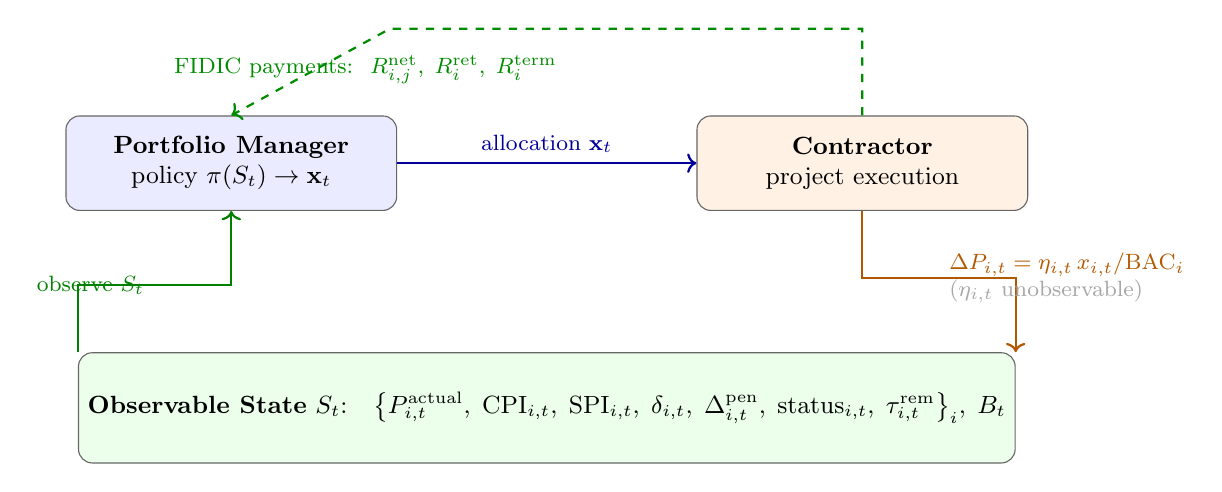
\begin{tikzpicture}[
    node distance=1.8cm,
    box/.style={rectangle, rounded corners=5pt, draw=black!60,
                fill=blue!8, minimum width=4.2cm,
                minimum height=1.2cm, align=center, font=\small},
    env/.style={rectangle, rounded corners=5pt, draw=black!60,
                fill=orange!10, minimum width=4.2cm,
                minimum height=1.2cm, align=center, font=\small},
    obs/.style={rectangle, rounded corners=5pt, draw=black!60,
                fill=green!8, minimum width=10.2cm,
                minimum height=1.4cm, align=center, font=\small},
    arr/.style={->, thick},
    ]

    \node[box] (pm)
    {\textbf{Portfolio Manager}\\policy $\pi(S_t) \to \mathbf{x}_t$};

    \node[env, right=3.8cm of pm] (contractor)
    {\textbf{Contractor}\\project execution};

    \node[obs, below=2.4cm of $(pm)!0.5!(contractor)$] (state)
    {\textbf{Observable State} $S_t$:\quad
        $\bigl\{P_{i,t}^{\mathrm{actual}},\;
        \mathrm{CPI}_{i,t},\;\mathrm{SPI}_{i,t},\;
        \delta_{i,t},\;\Delta_{i,t}^{\mathrm{pen}},\;
        \mathrm{status}_{i,t},\;\tau_{i,t}^{\mathrm{rem}}\bigr\}_{i},\;B_t$};

    \draw[arr, blue!60!black] (pm.east) -- (contractor.west)
    node[midway, above, font=\footnotesize] {allocation $\mathbf{x}_t$};

    \draw[arr, orange!70!black]
    (contractor.south) -- ++(0,-0.85) -| (state.north east)
    node[near start, right, font=\footnotesize, align=left]
        {$\Delta P_{i,t} = \eta_{i,t}\,x_{i,t}/\mathrm{BAC}_i$\\
        \textcolor{gray!70}{($\eta_{i,t}$ unobservable)}};

    \draw[arr, green!50!black]
    (state.north west) -- ++(0,0.85) -| (pm.south)
    node[near start, left, font=\footnotesize] {observe $S_t$};

    \draw[arr, dashed, green!55!black]
    (contractor.north) -- ++(0,1.1)
    -- ++(-6.0,0)
    -- (pm.north)
    node[near end, above, font=\footnotesize, green!55!black, xshift=1.2cm]
        {FIDIC payments:\;
        $R_{i,j}^{\mathrm{net}},\;R_i^{\mathrm{ret}},\;R_i^{\mathrm{term}}$};

\end{tikzpicture}
\caption{Portfolio governance feedback loop. The portfolio manager (agent)
    controls only the budget allocation vector $\mathbf{x}_t$. Contractors
    convert allocations into physical progress through efficiency $\eta_{i,t}$,
    which is unobservable and realized only after commitment. The full state
    $S_t$ is observable each period; FIDIC milestone payments, retention
    release, and termination settlement flow back as cash inflows.}
\label{fig:feedback_loop}
\end{figure}

\paragraph{Project execution.}
At the project level, the contractor controls workforce, materials, equipment,
and subcontracting. The portfolio manager observes the outcomes of these
decisions --- cumulative progress, earned value, payment certifications ---
but does not control them. The efficiency with which a budget allocation is
converted into physical progress is determined at the project level and is
uncertain from the portfolio manager's perspective.

This hierarchy is central to the modelling architecture: the formulation
developed in Section~\ref{sec:problem_formulation} lives entirely at the
portfolio governance layer, with project execution dynamics appearing only as
parameters (deterministic at Level~1, stochastic at Levels~2 and~3).

% ------------------------------------------------------------
\subsection{Contract Mechanics and Cash-Flow Structure}
\label{subsec:contract_mechanics}
% ------------------------------------------------------------

The financial interaction between the portfolio manager (as client) and each
contractor is governed by the contract. This paper parameterises all contract
mechanics consistently with FIDIC Red, Yellow, and Silver Book forms
\citep{FIDIC2017}, which represent the dominant international framework for
EPC contracting. Understanding the cash-flow structure is essential to
understanding the optimisation problem; this subsection provides that
foundation.

\paragraph{Milestone-based payment.}
Rather than paying contractors on a time-basis, FIDIC contracts structure
payment around certified milestones: discrete progress thresholds at which the
client verifies that a specified scope fraction has been physically completed
and releases the corresponding payment. The gross payment at milestone $j$ is a
contractually fixed fraction $\phi_{i,j}$ of the contract price $CP_i$.
Because payment is contingent on certified progress, the timing of cash
inflows is a function of the contractor's actual performance and, through the
portfolio manager's allocation decisions, of the budget directed to the project.
This creates the fundamental linkage between allocation decisions and cash
inflows that makes the problem non-trivial.

\paragraph{Advance payment and progressive recovery.}
At project initiation, the client disburses an advance payment $A_i =
\alpha_i \cdot CP_i$ to the contractor. This is a timing instrument: it
reduces the contractor's early working-capital burden and is recovered
progressively through percentage deductions from subsequent interim payment
certificates, with the deduction rate $\delta_i^{\mathrm{rec}}$ and
commencement threshold $\psi_i$ specified as project-specific contract
parameters \citep{FIDIC2017}. The advance payment creates an immediate cash inflow at project start and a
series of reduced inflows at each certified milestone, both of which must be
tracked in the portfolio cash balance. Interim milestone payments are
additionally subject to stochastic timing delays between certification and
receipt, consistent with observed payment practices in international EPC
contracting \citep{Aibinu2006, Odeh2002}; the amount transferred equals the
contractually fixed net milestone value, but the period of receipt is a random
variable.

\paragraph{Retention.}
A fraction $\rho_i$ of each milestone payment is withheld by the client as a
performance bond. The accumulated retention $R_i^{\mathrm{ret}} = \rho_i
\cdot CP_i$ is released in full upon project completion. Retention creates a
structural completion incentive embedded in the payment mechanics: the larger
the retention fraction, the more strongly the cash flow profile rewards
completion over partial delivery. In the formulation, retention release enters
the portfolio cash balance as a lump inflow in the period the final milestone
is certified.

\paragraph{Earned value management as a performance signal.}
The Earned Value Management framework \citep{Fleming2010} provides the
diagnostic vocabulary used to monitor contractor performance. The Cost
Performance Index $\mathrm{CPI}_{i,t} = \text{BCWP}_{i,t} /
\text{ACWP}_{i,t}$ measures how much budgeted value has been earned per unit
of actual expenditure; values below unity indicate cost overrun. The Schedule
Performance Index $\mathrm{SPI}_{i,t} = \text{BCWP}_{i,t} /
\text{BCWS}_{i,t}$ measures actual progress relative to planned progress;
values below unity indicate schedule lag \citep{Fleming2010}. In the present
formulation, these indices are observable state variables that inform the
allocation decision; their stochastic dynamics at Levels~2 and~3 are
calibrated from empirical EVM datasets \citep{Acebes2015, Batselier2017}.

\paragraph{S-curve expenditure profiles.}
The planned expenditure of a construction or engineering project follows a
characteristic sigmoid profile over its planned duration: slow ramp-up in the
mobilisation phase, rapid expenditure in the peak execution phase, and tapering
in the close-out phase \citep{Kenley2009}. This profile is modelled using the
regularized incomplete Beta function $F_i(\tau) = I_\tau(a_i, b_i)$, whose
shape parameters $(a_i, b_i)$ are calibrated from project data. The planned
cumulative expenditure fraction at normalised time $\tau_{i,t}$ provides the
baseline against which actual progress is measured throughout the formulation.

\paragraph{Termination.}
FIDIC contracts provide for client-initiated termination when the contractor
has materially breached the contract --- most commonly through sustained failure
to meet schedule obligations. Termination triggers a settlement payment based
on the value of work completed at the termination date, net of any outstanding
advance recovery obligation. In the present model, termination is an endogenous environment mechanic, not a
deliberate agent action. It is triggered when two conditions hold simultaneously
for a project-specific number of consecutive periods --- the termination
tolerance $\tau_i^{\mathrm{tol}}$: the forecast finish deviation has exceeded
the contractual penalty ceiling, and the cost performance index has fallen below
a project-specific recovery threshold $\kappa_i$. This joint persistence
requirement models the FIDIC cure period \citep{FIDIC2017, Ndekugri2008}, the
contractually prescribed interval during which both parties are obliged to
attempt performance recovery before the client may formally terminate. The
tolerance counter $\tau_{i,t}^{\mathrm{rem}}$ --- periods remaining before
termination executes --- is part of the observable environment state; the agent
cannot override its dynamics but observes its value and can influence it
indirectly through allocation decisions that affect $\mathrm{SPI}_{i,t}$ and
$\mathrm{CPI}_{i,t}$. When the counter reaches zero, termination executes in
the following period, and its timing affects the portfolio cash balance through
the settlement payment $R_i^{\mathrm{term}}$, which may be positive or negative
depending on the advance recovery position.

\begin{figure}[htbp]
\centering
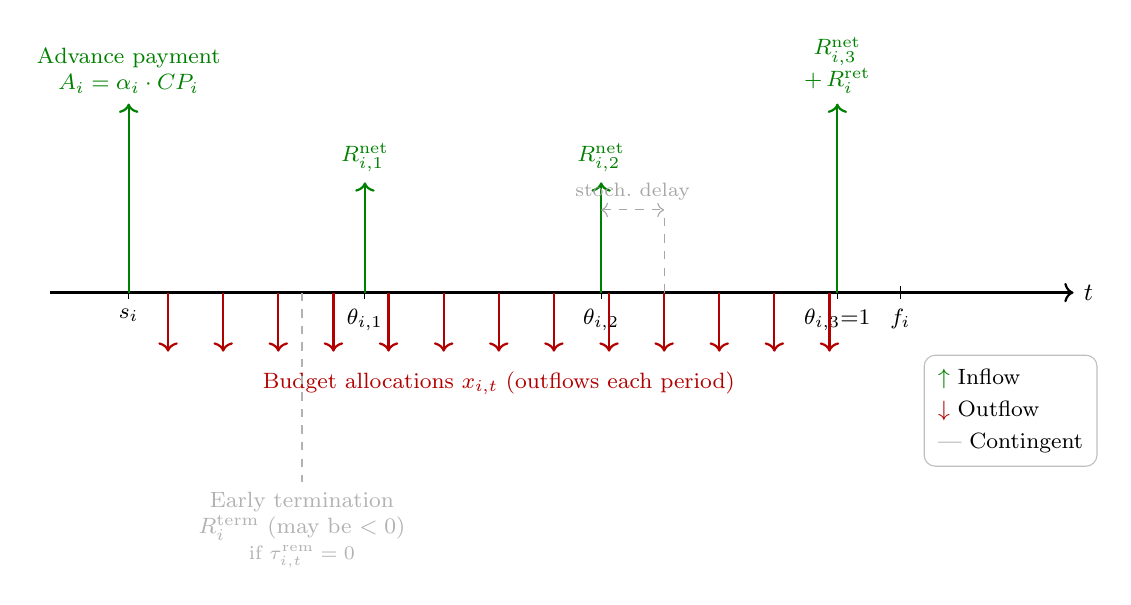
\begin{tikzpicture}[
    every node/.style={font=\small},
    inflow/.style={->, thick, green!50!black},
    outflow/.style={->, thick, red!70!black},
    ]

    \draw[->, thick] (0,0) -- (13.0,0) node[right] {$t$};

    \foreach \x/\lbl in {1/$s_i$, 4/$\theta_{i,1}$, 7/$\theta_{i,2}$,
                        10/$\theta_{i,3}{=}1$, 10.8/$f_i$}{
    \draw (\x,0.08) -- (\x,-0.08)
        node[below, font=\footnotesize] {\lbl};
    }

    \draw[inflow] (1,0) -- (1,2.4)
    node[above, align=center, font=\footnotesize]
        {Advance payment\\$A_i = \alpha_i \cdot CP_i$};

    \draw[inflow] (4,0) -- (4,1.4)
    node[above, font=\footnotesize] {$R_{i,1}^{\mathrm{net}}$};
    \draw[inflow] (7,0) -- (7,1.4)
    node[above, font=\footnotesize] {$R_{i,2}^{\mathrm{net}}$};

    \draw[<->, dashed, gray!70] (7,1.05) -- (7.8,1.05)
    node[midway, above, font=\scriptsize, gray!70] {stoch.\ delay};
    \draw[dashed, gray!70] (7.8,0) -- (7.8,1.05);

    \draw[inflow] (10,0) -- (10,2.4)
    node[above, align=center, font=\footnotesize]
        {$R_{i,3}^{\mathrm{net}}$\\$+\,R_i^{\mathrm{ret}}$};

    \foreach \x in {1.5,2.2,2.9,3.6,4.3,5.0,5.7,6.4,7.1,7.8,8.5,9.2,9.9}{
    \draw[outflow] (\x,0) -- (\x,-0.75);
    }
    \node[red!70!black, font=\footnotesize]
    at (5.7,-1.15) {Budget allocations $x_{i,t}$ (outflows each period)};

    \draw[dashed, thick, gray!60] (3.2,0) -- (3.2,-2.4)
    node[below, align=center, font=\footnotesize, gray!60]
        {Early termination\\$R_i^{\mathrm{term}}$ (may be $<0$)\\
        {\scriptsize if $\tau_{i,t}^{\mathrm{rem}}=0$}};

    \node[draw=gray!50, rounded corners, inner sep=5pt,
        align=left, font=\footnotesize] at (12.2,-1.5) {
    \textcolor{green!50!black}{$\uparrow$} Inflow\\[2pt]
    \textcolor{red!70!black}{$\downarrow$} Outflow\\[2pt]
    \textcolor{gray}{---} Contingent
    };

\end{tikzpicture}
\caption{Cash-flow timeline for project $i$ under FIDIC contract mechanics.
    The advance payment and milestone inflows are received from the client;
    budget allocations are disbursed each period. Milestone payments are
    subject to stochastic timing delays between certification and receipt.
    The dashed branch illustrates the termination settlement path if the
    cure-period counter reaches zero before project completion.}
\label{fig:cashflow_timeline}
\end{figure}

% ------------------------------------------------------------
\subsection{The Three-Level Modelling Arc}
\label{subsec:three_levels}
% ------------------------------------------------------------

The formulation of Section~\ref{sec:problem_formulation} proceeds across three
levels of increasing generality. This subsection provides the conceptual
roadmap; each level is developed formally in its corresponding subsection.

\paragraph{Level~1: Deterministic full-foresight MILP.}
The natural starting point for any optimisation problem is its deterministic
version: assume all uncertain parameters are known, and find the optimal
decision sequence. In the portfolio budget allocation problem, the key
uncertain parameter is the budget-to-progress efficiency $\eta_{i,t}$ ---
the scalar that determines how much physical progress a given budget allocation
yields in each period. If $\eta_{i,t}$ is treated as a known constant
$\bar{\eta}_{i,t}$, the progress recursion becomes a deterministic linear map
from budget allocations to physical outcomes, and the entire optimisation
problem collapses to a Mixed-Integer Linear Program (MILP).

The MILP is not proposed as a practical solution method --- no real portfolio
manager has advance knowledge of contractor efficiency trajectories. Rather,
it serves two purposes. First, its optimal value $Z^*_{\mathrm{L1}}$ is a
provable upper bound on the performance of any causal policy operating under
uncertainty: since the MILP optimises with perfect foresight, it can do no
worse than any policy that must make decisions without knowing future outcomes.
Second, it provides an LP foundation from which the stochastic extensions of
Levels~2 and~3 are constructed by systematic relaxation of the deterministic
assumption.

The MILP requires two structural choices that are standard in combinatorial
optimisation. Milestone certification is a binary event --- a milestone is
either certified or not --- captured by introducing binary decision variables
$u_{i,j,t} \in \{0,1\}$. The symmetric running deviation penalty involves an
absolute value and a cap, both of which are linearised by introducing auxiliary
variables $d_{i,t}^+, d_{i,t}^- \geq 0$ for the positive and negative parts of
the deviation. These linearisations are exact: no approximation is introduced. A third
structural feature is the termination mechanic: under deterministic
$\bar{\eta}_{i,t}$, both termination conditions and the tolerance counter
trajectory $\tau_{i,t}^{\mathrm{rem}}$ are fully pre-computable, so
termination periods $t_i^{\mathrm{term}}$ and their settlements
$R_i^{\mathrm{term}}$ enter the MILP as fixed parameters rather than
optimisation constraints --- a simplification that does not carry over to
Levels~2 and~3, where termination timing is endogenous to the stochastic
trajectory.

\paragraph{Level~2: Stochastic extension and intractability.}
When $\eta_{i,t}$ is replaced by a random variable --- as it must be to reflect
reality --- the MILP becomes a multi-stage stochastic program
\citep{Birge2011}. The scenario-tree representation of this program grows
exponentially: if $\eta_{i,t}$ takes $K$ discrete values at each of $H$
periods for each of $n$ projects, the scenario tree has $K^{nH}$ leaf nodes.
For a portfolio of ten projects over a 24-month horizon with five efficiency
scenarios per project per period, this is $5^{240}$ leaf nodes --- a number
that renders exact stochastic programming computationally intractable. This is
not merely a computational inconvenience; it is the fundamental barrier that
motivates the Level~3 reformulation.

\paragraph{Level~3: Constrained MDP and RL agent.}
The Constrained Markov Decision Process \citep{Altman1999} provides the
tractable reformulation. Rather than optimising over all scenario-tree paths
simultaneously, the CMDP formalises the problem as a sequential interaction
between a policy and an environment: at each period, the policy observes the
current portfolio state, selects a budget allocation, and the environment
transitions stochastically to the next state. The key insight is that the
CMDP does not require explicit scenario enumeration: the policy is optimised
through repeated interaction with the environment, using sampled trajectories
rather than exhaustive scenario trees.

The mapping from MILP to CMDP is exact in structure. The decision variables
$\{x_{i,t}\}$ become the action space; the state variables $(P_{i,t}^{\rm
actual}, E_{i,t}, \mathrm{CPI}_{i,t}, \mathrm{SPI}_{i,t}, \delta_{i,t},
\Delta_{i,t}^{\rm pen}, \mathrm{status}_{i,t}, \tau_{i,t}^{\mathrm{rem}},
B_t)$ become the observation
space; and the
objective function becomes the reward signal. The CMDP is implemented as a
configurable Gymnasium-compatible environment \citep{Towers2024}, and a
Proximal Policy Optimisation agent \citep{Schulman2017} is trained on it using
domain randomisation \citep{Tobin2017} to ensure generalisation across project
types and contract structures.

% ------------------------------------------------------------
\subsection{The Operations Research Lineage}
\label{subsec:or_lineage}
% ------------------------------------------------------------

The present work is situated squarely within the Industrial Engineering and
Operations Research tradition. The mathematical tools employed ---
mixed-integer linear programming, stochastic programming, dynamic programming,
and Markov decision processes --- share a common intellectual lineage that
traces directly to Dantzig's simplex method \citep{Dantzig1963}, Bellman's
principle of optimality \citep{Bellman1957}, and the stochastic programming
framework of \citet{Dantzig1955}.

The MDP formalisation used in Level~3 is, mathematically, a computationally
tractable approach to solving a Bellman equation in a high-dimensional state
space. The state space in the present problem --- $8n + 1$ continuous and
categorical variables for a portfolio of $n$ projects --- is too large for
tabular dynamic programming and too structured for model-free value-iteration
methods, but well-suited to policy-gradient methods that learn a parameterised
policy directly. PPO \citep{Schulman2017} is the policy-gradient algorithm of
choice for its stability properties in continuous action spaces and its
established use in operations management domains \citep{Giannoccaro2002,
Peng2021}.

The reinforcement learning agent is therefore not presented as a departure from
the OR tradition, but as its continuation into the regime where the curse of
dimensionality makes analytical dynamic programming intractable. The Level~1
MILP and Level~2 stochastic program are not straw men; they are the canonical
OR solutions to the deterministic and stochastic versions of the problem,
respectively, and both serve as baselines against which the Level~3 agent is
evaluated.

% ------------------------------------------------------------
\subsection{Practical Deployment Context}
\label{subsec:deployment}
% ------------------------------------------------------------

Incumbent project management information systems --- most prominently Oracle
Primavera P6 and Microsoft Project --- provide rich project-level schedule and
cost tracking but lack a portfolio-level optimisation layer. The portfolio
manager's recurring budget allocation decision is currently supported, at best,
by spreadsheet models, earned value dashboards, and expert judgement. The
environment developed in Level~3 constitutes the analytical engine that such a
portfolio-level decision-support module would require: it integrates contract
mechanics, performance uncertainty, and multi-project cash-flow dynamics in a
single configurable framework. This positions the contribution not only as a
theoretical advance but as a step toward a deployable module for portfolio
management information systems, a direction explicitly identified as a priority
in the project management software literature \citep{PMI2017}.

% ------------------------------------------------------------
\subsection{Paper Organisation}
\label{subsec:organisation}
% ------------------------------------------------------------

The remainder of the paper is organised as follows.
Section~\ref{sec:litreview} reviews the four literature streams on which the
work draws: project management foundations, project portfolio management and
selection, PPM budgeting and cash-flow modelling, and reinforcement learning
for sequential resource allocation.
Section~\ref{sec:problem_formulation} develops the three-level problem
formulation: the deterministic MILP (Level~1), the stochastic extension and
intractability argument (Level~2), and the CMDP reformulation and
Gymnasium-compatible environment (Level~3).
Section~\ref{sec:experiments} presents the empirical evaluation: calibration
of environment parameters, training protocol, and comparison of the PPO agent
against the Level~1 MILP oracle, a two-stage stochastic program, and a
rule-based heuristic.
Section~\ref{sec:conclusion} concludes with implications for portfolio
management practice, limitations of the framework, and directions for future
research including integration with incumbent PMIS tools.

\FloatBarrier

% ============================================================
%  LITERATURE REVIEW
% ============================================================

\section{Literature Review}
\label{sec:literature}
\subsection{Project Portfolio Management Under Uncertainty}

Project portfolio management (PPM) has been extensively studied in operations research and management science. Early work by \citet{archer1999integrated} established frameworks for project selection and prioritization, while \citet{cooper2001portfolio} developed stage-gate processes for new product development portfolios. However, these approaches primarily address the \textit{selection} problem (which projects to pursue) rather than the \textit{execution} problem (how to allocate resources dynamically).

\citet{gutjahr2008project} formulated multi-objective portfolio optimization models balancing expected return, risk, and strategic alignment. \citet{doerner2006pareto} applied Pareto ant colony optimization to generate efficient frontiers for portfolio selection. These methods assume deterministic project execution once selected, ignoring the sequential decision-making required under performance uncertainty.

Stochastic programming approaches have been proposed to handle uncertainty. \citet{golenko1997stochastic} modeled resource-constrained project scheduling with stochastic activity durations. \citet{klerides2019stochastic} developed two-stage stochastic programs for portfolio selection under demand uncertainty. However, these methods require explicit scenario trees and known probability distributions, which are unavailable for contractor performance dynamics.

\subsection{Project Performance Uncertainty and Empirical Evidence}

A substantial body of empirical research documents systematic cost and schedule overruns in capital projects. \citet{flyvbjerg2002underestimating} analyzed 258 transportation infrastructure projects, finding mean cost overruns of 28\% and schedule delays of 27\%. \citet{flyvbjerg2003underestimating} extended this analysis to 258 projects across multiple sectors, confirming left-skewed performance distributions with long tails toward poor outcomes.

\citet{merrow2011industrial} provided the most comprehensive analysis of EPC project performance, examining 318 industrial megaprojects in oil \& gas, chemicals, and mining. Key findings include: (1) mean SPI at completion of 0.81 (19\% behind schedule), (2) mean CPI of 0.87 (15\% over budget), (3) positive correlation between schedule and cost performance ($\rho \approx 0.68$), and (4) systematic variation in performance by project size, complexity, and contractor experience.

\citet{love2013probability} fitted probability distributions to schedule overrun data from 276 construction projects, validating Beta and lognormal distributions as appropriate models. \citet{love2016relationship} analyzed the relationship between SPI and CPI, confirming that schedule delays typically precede cost overruns due to extended overhead and acceleration costs.

\subsection{Cashflow Modeling and S-Curves}

Project cashflow modeling has a rich history in construction management. \citet{kenley1986construction} introduced the idiographic approach to cashflow forecasting, recognizing that each project exhibits unique spending patterns. \citet{kaka1993towards} developed neural network models for cashflow prediction based on historical project data.

The S-curve model, representing cumulative spending as a sigmoid function of project duration, has become the standard representation. \citet{cioffi2005tool} provided analytical parameterization of S-curves using Beta distributions, enabling closed-form expressions for cashflow velocity and peak spending timing. \citet{barraza2007probabilistic} extended this to probabilistic S-curves incorporating uncertainty in project duration and spending patterns.

\citet{cui2010systems} analyzed milestone-based payment structures in construction contracts, finding that 87\% of contracts use progress-based payments rather than time-based schedules. This finding motivates our modeling choice to link payment timing to actual progress (SPI) rather than calendar dates.

\subsection{Reinforcement Learning in Operations Research}

RL has emerged as a powerful tool for sequential decision-making under uncertainty. \citet{sutton2018reinforcement} provide the foundational textbook covering Markov Decision Processes (MDPs), temporal difference learning, and policy gradient methods. Recent advances in deep RL, particularly Proximal Policy Optimization (PPO) \citep{schulman2017proximal} and Soft Actor-Critic (SAC) \citep{haarnoja2018soft}, have enabled application to high-dimensional continuous control problems.

Applications of RL to operations research problems have grown rapidly. \citet{hubbs2020deep} applied deep RL to chemical production scheduling, achieving near-optimal solutions with 1000× speedup over MIP. \citet{bengio2021machine} surveyed machine learning for combinatorial optimization, highlighting RL's ability to learn heuristics that generalize across problem instances.

In project management, RL applications remain limited. \citet{wauters2016learning} used RL for resource-constrained project scheduling with deterministic durations. \citet{chen2018reinforcement} applied RL to construction project scheduling under resource uncertainty. However, no prior work addresses portfolio-level budgeting under cashflow uncertainty with stochastic contractor performance.

\subsection{Synthetic Data Generation for OR/ML Research}

The use of synthetic data in operations research has a long tradition. \citet{kolisch1997psplib} created the Project Scheduling Problem Library (PSPLIB), a benchmark dataset of synthetic instances that became the standard for algorithm comparison. \citet{vanhoucke2008experimental} generated synthetic project networks to study schedule risk analysis methods.

In machine learning, synthetic data generation has become essential for domains with data scarcity or privacy constraints. \citet{jordon2022synthetic} surveyed synthetic data generation methods, emphasizing the importance of preserving statistical properties of real data. \citet{xu2019modeling} developed generative models for tabular data that maintain correlations and distributional characteristics.

For project management, \citet{vanhoucke2012integrated} generated synthetic project data with controlled complexity levels to benchmark scheduling algorithms. \citet{elshaer2014genetic} created synthetic portfolios with varying risk profiles to test portfolio optimization methods. Our work extends this tradition by developing a comprehensive synthetic data generator calibrated to empirical distributions from multiple literature sources, ensuring realism while maintaining reproducibility.

\subsection{Research Gaps}

Despite extensive research in project portfolio management, performance uncertainty, and RL applications, critical gaps remain:

\begin{enumerate}
    \item \textbf{No RL framework for portfolio budgeting:} Existing RL applications to project management focus on single-project scheduling, not portfolio-level resource allocation under cashflow uncertainty.
    
    \item \textbf{Lack of realistic synthetic environments:} Prior synthetic data generators for project management do not model stochastic contractor performance, milestone-based payments, or portfolio-level cashflow dynamics.
    
    \item \textbf{Absence of rolling horizon RL architectures:} Rolling horizon control has not been integrated with RL for portfolio management, despite its natural fit for handling variable-duration portfolios.
    
    \item \textbf{No methodology for literature-calibrated data generation:} Existing approaches either use proprietary data (unavailable for research) or arbitrary synthetic distributions (lacking empirical grounding).
\end{enumerate}

This paper addresses these gaps by developing the first RL framework for portfolio budgeting with a literature-calibrated synthetic environment and rolling horizon architecture.


\FloatBarrier

% ============================================================
%  PROBLEM FORMULATION
% ============================================================

\section{Problem Formulation}
\label{sec:problem}
% ============================================================
%  SECTION 3 — PROBLEM FORMULATION
% ============================================================
This section develops the formal problem structure for portfolio-level budget
allocation in contracted project portfolios. The formulation proceeds across
three levels. \textbf{Level~1} (Section~\ref{subsec:level1}) treats all
contractor performance parameters as known and establishes the deterministic
MILP whose optimum constitutes a theoretical upper bound: no implementable
policy operating under uncertainty can exceed it.
\textbf{Level~2} (Section~\ref{subsec:level2}) reintroduces stochastic
efficiency and characterizes the resulting multi-stage stochastic program,
establishing that its scenario tree grows exponentially in the number of
projects and periods. \textbf{Level~3} (Section~\ref{subsec:level3})
reformulates the intractable stochastic program as a Constrained Markov
Decision Process (CMDP), providing an explicit mapping from LP elements to MDP
primitives and yielding a Gymnasium-compatible environment on which the PPO
agent of Section~\ref{sec:experiments} is trained. The three levels are a
coherent arc --- Level~1 defines the ceiling, Level~2 explains why it is
unreachable, Level~3 provides the tractable path --- all sharing the primitives
defined next.

% ------------------------------------------------------------
\subsection{Scope, Assumptions, and Problem Primitives}
\label{subsec:primitives}
% ------------------------------------------------------------

\paragraph{Scope.}
The problem is operational, not strategic: the portfolio of contracted projects
is fixed, commitments are signed, and the decision-maker exercises a single
lever --- the budget $x_{i,t}$ directed to each active project $i$ at each
discrete period $t$. All outcomes of interest (milestone achievement, cash
balance, schedule adherence, termination) flow through this allocation decision.
Portfolio selection is treated as exogenous \cite{Archer1999}.

\paragraph{Structural assumptions.}
Four choices underlie the entire formulation.
(i)~\emph{Independent bilateral contracts}: projects interact only through the
shared budget constraint; no resource or workforce sharing occurs, consistent
with standard EPC contracting practice.
(ii)~\emph{Budget as the sole control}: the contractor's internal resource
decisions are absorbed into the efficiency parameter $\eta_{i,t}$; the
portfolio manager observes only how much physical progress a budget allocation
yields, not how it is achieved.
(iii)~\emph{Discrete monthly periods}: $\mathcal{T} = \{1,\ldots,H\}$
reflects the monthly governance cycle of portfolio management (progress
reporting, payment certification, performance review).
(iv)~\emph{FIDIC contract mechanics}: the milestone payment structure, advance
payment and recovery, retention, and termination settlement are parameterized
consistently with FIDIC Red, Yellow, and Silver Book forms
\cite{FIDIC2017}; all contract-specific quantities are calibrated
parameters, not fixed constants.

% - - - - - - - - - - - - - - - - - - - - - - - - - - - - - -
\subsubsection{Sets, Indices, and the Decision Variable}
\label{subsubsec:sets}
% - - - - - - - - - - - - - - - - - - - - - - - - - - - - - -

\begin{description}[leftmargin=2.2cm, labelwidth=2.0cm]
  \item[$\mathcal{P}$]
    Projects $\{1,\ldots,n\}$, indexed by $i$; all committed at horizon start.
  \item[$\mathcal{T}$]
    Planning periods $\{1,\ldots,H\}$, indexed by $t$ (calendar months).
  \item[$\mathcal{M}_i$]
    Ordered milestones $\{1,\ldots,M_i\}$ for project $i$, indexed by $j$,
    with thresholds $\theta_{i,1} < \cdots < \theta_{i,M_i} = 1$.
  \item[$\mathcal{A}_i^{\mathrm{plan}}$]
    Planned execution window $\{s_i,\ldots,f_i\}$; anchors S-curve computations.
  \item[$\mathcal{P}_t^{\mathrm{active}}$]
    Projects active at period $t$; fixed parameter at Level~1, endogenous at
    Levels~2--3.
  \item[$\mathcal{M}_i^{\mathrm{cert}}(t)$]
    Milestones of project $i$ certified by period $t$:
    $\{j : \theta_{i,j} \leq P_{i,t}^{\mathrm{actual}}\}$.
  \item[$x_{i,t} \geq 0$]
    \textbf{Decision variable}: budget allocated to project $i$ at period $t$.
    The period-$t$ action is $\mathbf{x}_t = (x_{i,t})_{i \in
    \mathcal{P}_t^{\mathrm{active}}}$.
  \item[$B_t \geq 0$]
    Portfolio cash balance at the start of period $t$; $B_1$ is given.
\end{description}

% - - - - - - - - - - - - - - - - - - - - - - - - - - - - - -
\subsubsection{Project Parameters}
\label{subsubsec:project_params}
% - - - - - - - - - - - - - - - - - - - - - - - - - - - - - -

Tables~\ref{tab:params-schedule-contract} and~\ref{tab:params-cost-penalty}
list all project parameters, fixed at commitment. The planned cumulative
expenditure fraction follows a normalized S-curve
\cite{Kenley2009,barraza2004probabilistic} parameterized by
$(a_i,b_i)$:
\[
  P_{i,t}^{\mathrm{plan}} = F_i(\tau_{i,t}^c) = I_{\tau_{i,t}^c}(a_i, b_i),
  \qquad
  \tau_{i,t} = \frac{t - s_i + 1}{D_i^{\mathrm{plan}}},
  \quad
  \tau_{i,t}^c = \min\{1,\max\{0,\tau_{i,t}\}\},
\]
where $I_\tau(\cdot,\cdot)$ is the regularized incomplete Beta function.
The planned period expenditure increment is
$\Delta\bar{E}_{i,t} = \mathrm{BAC}_i\,[F_i(\tau_{i,t}^c) - F_i(\tau_{i,t-1}^c)]$.
This profile is a fixed parameter derived at commitment from
$(a_i, b_i, s_i, f_i, \mathrm{BAC}_i)$; it is never a decision variable.

\begin{table}[H]
  \centering\small
  \renewcommand{\arraystretch}{1.3}\setlength{\tabcolsep}{8pt}
  \begin{tabular}{>{\bfseries}p{3.4cm} p{2.0cm} p{1.3cm} p{7.0cm}}
    \toprule
    \normalfont\textbf{Parameter} & \textbf{Symbol} & \textbf{Domain} & \textbf{Definition} \\
    \midrule
    \rowcolor{RowAlt}
    Planned start \& finish \newline\tagschedule
      & $s_i,\;f_i$ & $\mathbb{Z}^+$
      & Anchor of execution window $\mathcal{A}_i^{\mathrm{plan}}$ and S-curve. \\
    Planned duration \newline\tagschedule
      & $D_i^{\mathrm{plan}}$ & $\mathbb{Z}^+$
      & $f_i - s_i + 1$; normalizes progress against plan. \\
    \rowcolor{RowAlt}
    S-curve shape \newline\tagschedule
      & $a_i,\;b_i$ & $\mathbb{R}^+$
      & Beta CDF parameters governing the planned expenditure profile. \\
    Milestone threshold \newline\tagschedule
      & $\theta_{i,j}$ & $(0,1]$
      & Cumulative progress fraction required to certify milestone $j$. \\
    \rowcolor{RowAlt}
    Delay buffer \newline\tagschedule
      & $\mathrm{buffer}_i$ & $\mathbb{Z}^+_0$
      & Periods beyond $f_i$ before forced termination is assessed. \\
    \midrule
    Contract price \newline\tagcontract
      & $CP_i$ & $\mathbb{R}^+$
      & Total client payment; $CP_i = \mathrm{BAC}_i(1+\pi_i)$. \\
    \rowcolor{RowAlt}
    Profit margin \newline\tagcontract
      & $\pi_i$ & $\mathbb{R}^+_0$
      & Contractual markup on $\mathrm{BAC}_i$. \\
    Advance payment ratio \newline\tagcontract
      & $\alpha_i$ & $[0,1]$
      & $A_i = \alpha_i \cdot CP_i$ received at $t = s_i$; recovered through
        percentage deductions from subsequent interim payment certificates at
        rate $\delta_i^{\mathrm{rec}}$ once cumulative certified payments
        exceed threshold $\psi_i$ \citep{FIDIC2017}. \\
    \rowcolor{RowAlt}
    Recovery deduction rate \newline\tagcontract
      & $\delta_i^{\mathrm{rec}}$ & $(0,1]$
      & Fraction of each interim payment certificate deducted toward advance
        recovery once the commencement threshold $\psi_i$ is exceeded. \\
    Recovery commencement threshold \newline\tagcontract
      & $\psi_i$ & $[0,1]$
      & Cumulative certified interim payments as a fraction of $CP_i$ at which
        advance recovery deductions begin; default 0.10 under FIDIC
        Sub-Clause~14.2 \citep{FIDIC2017}. \\
    \rowcolor{RowAlt}
    Retention ratio \newline\tagcontract
      & $\rho_i$ & $[0,1]$
      & Fraction withheld per milestone; released as $R_i^{\mathrm{ret}} = \rho_i \cdot CP_i$ at completion. \\
    Milestone weight \newline\tagcontract
      & $\phi_{i,j}$ & $\mathbb{R}^+$
      & Fraction of $CP_i$ at milestone $j$; $\sum_j \phi_{i,j} = 1$. \\
    \bottomrule
  \end{tabular}
  \caption{Schedule and contract parameters for project $i \in \mathcal{P}$ (fixed at commitment).}
  \label{tab:params-schedule-contract}
\end{table}

\begin{table}[H]
  \centering\small
  \renewcommand{\arraystretch}{1.3}\setlength{\tabcolsep}{8pt}
  \begin{tabular}{>{\bfseries}p{3.4cm} p{2.0cm} p{1.3cm} p{7.0cm}}
    \toprule
    \normalfont\textbf{Parameter} & \textbf{Symbol} & \textbf{Domain} & \textbf{Definition} \\
    \midrule
    \rowcolor{RowAlt}
    Budget at completion \newline\tagcost
      & $\mathrm{BAC}_i$ & $\mathbb{R}^+$
      & Total planned contractor expenditure; EVM cost basis. \\
    Discount factor \newline\tagcost
      & $\gamma$ & $(0,1]$
      & Per-period discount applied to future cash flows; shared across $\mathcal{P}$. \\
    \rowcolor{RowAlt}
    Initial cash balance \newline\tagcost
      & $B_1$ & $\mathbb{R}^+$
      & Portfolio cash balance at horizon start; initial condition of balance recursion. \\
    \midrule
    Deviation penalty weight \newline\tagpenalty
      & $\lambda_i$ & $\mathbb{R}^+_0$
      & Per-period cost per unit absolute progress deviation; calibrated so cumulative
        penalty at planned finish under sustained contractual-limit delay equals
        $\Lambda_i \cdot CP_i$. \\
    \rowcolor{RowAlt}
    Deviation penalty cap \newline\tagpenalty
      & $\Lambda_i$ & $\mathbb{R}^+_0$
      & Maximum cumulative penalty as fraction of $CP_i$; applies symmetrically to
        lag and acceleration. \\
    Per-period delay rate \newline\tagpenalty
      & $r_i$ & $\mathbb{R}^+_0$
      & Per-period penalty rate used in the forecast-deviation termination
        condition; $\Lambda_i / r_i$ gives the maximum tolerable delay in periods. \\
    \midrule
    \rowcolor{RowAlt}
    CPI recovery threshold \newline\tagterm
      & $\kappa_i$ & $(0,1)$
      & Project-specific CPI floor; $\mathrm{CPI}_{i,t} < \kappa_i$ signals
        cost performance is unrecoverable and activates Termination Condition~2. \\
    Termination tolerance \newline\tagterm
      & $\tau_i^{\mathrm{tol}}$ & $\mathbb{Z}^+$
      & Maximum number of consecutive periods both termination conditions may
        hold simultaneously before termination executes; models the FIDIC
        cure period \citep{FIDIC2017, Ndekugri2008}. \\
    \bottomrule
  \end{tabular}
  \caption{Cost, penalty, and termination parameters for project $i \in \mathcal{P}$ (fixed at commitment).}
  \label{tab:params-cost-penalty}
\end{table}

\begin{table}[htbp]
  \centering
  \caption{Parameter groups cross-referenced to model equations and formulation
    levels. All parameters are fixed at project commitment.}
  \label{tab:param_navigation}
  \renewcommand{\arraystretch}{1.35}
  \setlength{\tabcolsep}{7pt}
  \begin{tabular}{p{3.2cm} p{5.8cm} p{3.0cm} p{1.6cm}}
  \hline
  \textbf{Group} & \textbf{Parameters} & \textbf{Enters at} & \textbf{Level} \\
  \hline
  Schedule
    & $s_i,\; f_i,\; D_i^{\mathrm{plan}},\; a_i,\; b_i,\; \mathrm{buffer}_i$
    & \eqref{eq:progress_rec}, S-curve
    & 1, 2, 3 \\
  \rowcolor{RowAlt}
  Contract payments
    & $CP_i,\; \pi_i,\; \alpha_i,\; \delta_i^{\mathrm{rec}},\;
       \psi_i,\; \rho_i,\; \phi_{i,j}$
    & \eqref{eq:Rnet}, \eqref{eq:Vt}
    & 1, 2, 3 \\
  Deviation penalty
    & $\lambda_i,\; \Lambda_i,\; r_i$
    & \eqref{eq:penalty}, \eqref{eq:term_cond1}
    & 1, 2, 3 \\
  \rowcolor{RowAlt}
  Termination
    & $\kappa_i,\; \tau_i^{\mathrm{tol}}$
    & \eqref{eq:term_cond2}, \eqref{eq:counter}
    & 2, 3 \\
  Portfolio
    & $B_1,\; \gamma$
    & \eqref{eq:balance}, \eqref{eq:objective}
    & 1, 2, 3 \\
  \rowcolor{RowAlt}
  State variables
    & $\mathrm{CPI}_{i,t},\; \mathrm{SPI}_{i,t},\;
       \delta_{i,t},\; \Delta_{i,t}^{\mathrm{pen}},\;
       \tau_{i,t}^{\mathrm{rem}}$
    & $S_t$,\;\eqref{eq:counter}
    & 2, 3 \\
  \hline
  \end{tabular}
  \end{table}

% - - - - - - - - - - - - - - - - - - - - - - - - - - - - - -
\subsubsection{State Variables and Transition Dynamics}
\label{subsubsec:dynamics}
% - - - - - - - - - - - - - - - - - - - - - - - - - - - - - -

\paragraph{Project-level state.}
For each $i \in \mathcal{P}$, $t \in \mathcal{T}$:
$P_{i,t}^{\mathrm{actual}} \in [0,1]$ (cumulative progress),
$E_{i,t} \geq 0$ (cumulative expenditure),
$\mathrm{SPI}_{i,t} = P_{i,t}^{\mathrm{actual}} / P_{i,t}^{\mathrm{plan}}$,
$\mathrm{CPI}_{i,t} = P_{i,t}^{\mathrm{actual}} \cdot \mathrm{BAC}_i / E_{i,t}$,
$\delta_{i,t} = P_{i,t}^{\mathrm{actual}} - P_{i,t}^{\mathrm{plan}}$ (signed deviation),
$\Delta_{i,t}^{\mathrm{pen}} \geq 0$ (cumulative penalty),
$\mathrm{status}_{i,t} \in \{\texttt{active}, \texttt{completed}, \texttt{terminated}\}$,
and $\tau_{i,t}^{\mathrm{rem}} \in \{0,1,\ldots,\tau_i^{\mathrm{tol}}\}$
(periods remaining in the cure-period counter; zero triggers termination).
The portfolio state at period $t$ is:
\[
  S_t = \Bigl(
    \bigl\{P_{i,t}^{\mathrm{actual}},\, E_{i,t},\, \mathrm{SPI}_{i,t},\,
           \mathrm{CPI}_{i,t},\, \delta_{i,t},\, \Delta_{i,t}^{\mathrm{pen}},\,
           \mathrm{status}_{i,t},\, \tau_{i,t}^{\mathrm{rem}}\bigr\}_{i \in \mathcal{P}},\; B_t
  \Bigr).
\]

\paragraph{Budget-to-progress conversion.}
Budget $x_{i,t}$ converts to progress through the efficiency $\eta_{i,t}$:
\begin{equation}
  P_{i,t}^{\mathrm{actual}} = P_{i,t-1}^{\mathrm{actual}}
    + \eta_{i,t} \cdot \frac{x_{i,t}}{\mathrm{BAC}_i}, \qquad
  E_{i,t} = E_{i,t-1} + x_{i,t},
  \label{eq:progress_rec}
\end{equation}
with $P_{i,0}^{\mathrm{actual}} = E_{i,0} = 0$. The scalar $\eta_{i,t}$
absorbs all sources of conversion uncertainty (productivity, supply chain,
weather). At Level~1, $\eta_{i,t}$ is replaced by the known deterministic
value $\bar{\eta}_{i,t}$ (equal to unity under nominal plan); at Levels~2--3
it is a stochastic primitive realized only after $x_{i,t}$ is committed.

\paragraph{Contractual cash-flow mechanics.}
Payment inflows follow FIDIC mechanics \cite{FIDIC2017}. At initiation
($t = s_i$), the advance payment $A_i = \alpha_i \cdot CP_i$ is received.
Milestone $j$ is certified at the first $t$ with
$P_{i,t}^{\mathrm{actual}} \geq \theta_{i,j}$; the net payment (after
retention and advance recovery) is:
\begin{equation}
  R_{i,j}^{\mathrm{net}}
    = \phi_{i,j} \cdot CP_i (1 - \rho_i)
      - \delta_i^{\mathrm{rec}} \cdot \phi_{i,j} \cdot CP_i
        \cdot \mathbf{1}\!\left\{
          \sum_{k \leq j} \phi_{i,k} \geq \psi_i
        \right\}.
  \label{eq:Rnet}
\end{equation}
The second term deducts the advance recovery fraction $\delta_i^{\mathrm{rec}}$
from each milestone payment once cumulative certified payments have exceeded
the commencement threshold $\psi_i$, consistent with FIDIC Sub-Clause~14.2
\citep{FIDIC2017}. Upon completion ($P_{i,t}^{\mathrm{actual}} = 1$) the
accumulated retention $R_i^{\mathrm{ret}} = \rho_i \cdot CP_i$ is released
together with the final milestone payment. Aggregate period inflow is:
\begin{equation}
  V_t = \sum_{i,j} R_{i,j}^{\mathrm{net}}
          \cdot \mathbf{1}\{\text{$(i,j)$ newly certified at $t$}\}
        + \sum_{i \in \mathcal{P}_t^{\mathrm{term}}} R_i^{\mathrm{term}},
  \label{eq:Vt}
\end{equation}
where $\mathcal{P}_t^{\mathrm{term}}$ collects projects newly terminated at
$t$, with settlement $R_i^{\mathrm{term}}$ defined in
\eqref{eq:term_settlement} below. Milestone payments are subject to stochastic
timing delays between certification and receipt at Levels~2--3
\citep{Aibinu2006, Odeh2002}; the amount is fixed at the contractual net value
but the period of receipt is a random variable.

\FloatBarrier
\paragraph{Symmetric running deviation penalty.}
Schedule adherence is priced at every period:
\begin{equation}
  c_{i,t}^{\mathrm{dev}}
    = \min\!\bigl\{\lambda_i\,|\delta_{i,t}|,\; \Lambda_i \cdot CP_i\bigr\},
  \qquad
  \Delta_{i,t}^{\mathrm{pen}} = \sum_{\tau=s_i}^{t} c_{i,\tau}^{\mathrm{dev}}.
  \label{eq:penalty}
\end{equation}
The penalty is symmetric ($|\delta_{i,t}|$, not $\max\{0,-\delta_{i,t}\}$):
both lag and acceleration are penalized, discouraging budget-pushing that risks
quality degradation \cite{Merrow2011}. The cap $\Lambda_i \cdot CP_i$
mirrors the contractual delay-penalty ceiling under FIDIC terms.

\begin{figure}[htbp]
\centering
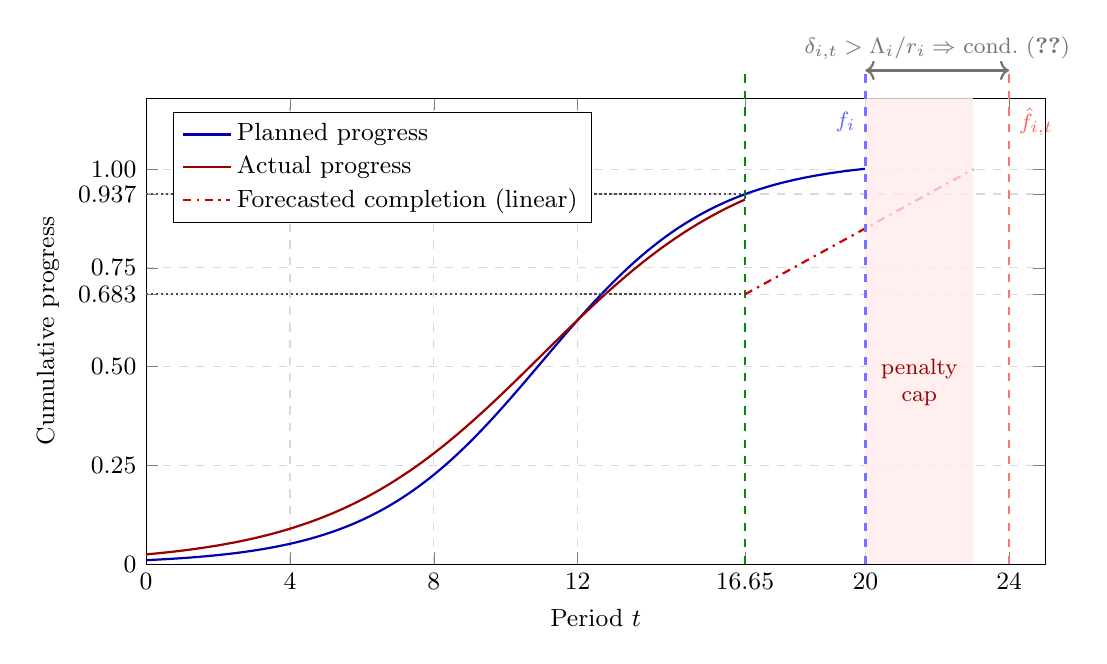
\begin{tikzpicture}
\begin{axis}[
    width=13cm, height=7.5cm,
    xlabel={Period $t$},
    ylabel={Cumulative progress},
    xmin=0, xmax=25,
    ymin=0, ymax=1.18,
    xtick={0,4,8,12,16.65,20,24},
    ytick={0,0.25,0.5,0.683,0.75,0.937,1.0},
    yticklabels={0,0.25,0.50,0.683,0.75,0.937,1.00},
    grid=major,
    grid style={dashed,gray!30},
    legend pos=north west,
    legend style={font=\small, cells={anchor=west}},
    tick label style={font=\small},
    label style={font=\small},
    clip=false,
  ]
  % ⚠️ this needs calibration. the actual curve must be expected to cross the threshold at an integer time

  \addplot[thick, blue!70!black, smooth, domain=0:20, samples=80]
    { (1/(1+exp(-0.42*(x-11)))) / 0.9767 };
  \addlegendentry{Planned progress}

  % \addplot[thick, red!60!black, smooth, domain=0:24, samples=80, dashed]
  %   { (0.88/(1+exp(-0.42*(x-15)))) / 0.860 };
  % \addlegendentry{Actual progress}
  
  \addplot[thick, red!60!black, smooth, domain=0:16.65, samples=80]
  { (1/(1+exp(-0.34*(x-11)))) / 0.945 };
  \addlegendentry{Actual progress}

  \draw[dashed, green!55!black, thick]
  (axis cs:16.65,0) -- (axis cs:16.65,1.25);

  \addplot[thick, red!80!black, dashdotted]
  coordinates {
    (16.65,0.683)
    (23,1)
  };
  \addlegendentry{Forecasted completion (linear)}

  \addplot[densely dotted, gray!60!black, thick]
  coordinates {(0,0.937)(16.65,0.937)};

  \addplot[densely dotted, gray!60!black, thick]
  coordinates {(0,0.683)(16.65,0.683)};
  
  \fill[red!8, opacity=0.8]
  (axis cs:20,0) rectangle (axis cs:23,1.18);
  \node[font=\footnotesize, red!60!black, align=center]
    at (axis cs:21.5,0.46)
    {penalty\\cap};

  \draw[dashed, blue!55, thick]
    (axis cs:20,0) -- (axis cs:20,1.25);
  \node[font=\footnotesize, blue!60, left]
    at (axis cs:20,1.12) {$f_i$};

  \draw[dashed, red!55, thick]
    (axis cs:24,0) -- (axis cs:24,1.25);
  \node[font=\footnotesize, red!60, right]
    at (axis cs:24,1.12) {$\hat{f}_{i,t}$};

  \draw[<->, thick, black!55]
    (axis cs:20,1.25) -- (axis cs:24,1.25)
    node[midway, above, font=\footnotesize]
      {$\delta_{i,t} > \Lambda_i/r_i \Rightarrow$ cond.~(\ref{eq:term_cond1})};

\end{axis}
\end{tikzpicture}
\caption{actual progress runs below, producing negative signed deviation $\delta_{i,t}$
  and values $\mathrm{SPI}_{i,t},\,\mathrm{CPI}_{i,t} < 1$. When the forecast
  finish gap $\hat{f}_{i,t}-f_i$ exceeds $\Lambda_i/r_i$ (shaded region),
  Termination Condition~(\ref{eq:term_cond1}) activates.}
\label{fig:scurve_evm}
\end{figure}

\FloatBarrier
\paragraph{Termination conditions and settlement.}
Termination is an endogenous environment mechanic. At each period $t$, the
environment evaluates two conditions for every active project $i$:
\begin{align}
  &\text{(i) Schedule tolerance exhausted:} \quad
    \hat{f}_{i,t} - f_i > \frac{\Lambda_i}{r_i},
  \label{eq:term_cond1} \\
  &\text{(ii) Cost performance unrecoverable:} \quad
    \mathrm{CPI}_{i,t} < \kappa_i,
  \label{eq:term_cond2}
\end{align}
where $\hat{f}_{i,t} = s_i + (D_i^{\mathrm{plan}} - (t - s_i)) /
\mathrm{SPI}_{i,t}$ is the linearly extrapolated forecast finish date and
$r_i$ is the per-period delay penalty rate. Condition~\eqref{eq:term_cond1}
signals that the forecast finish deviation has exceeded the maximum delay
the contract price can absorb before the penalty ceiling $\Lambda_i$ is
reached; Condition~\eqref{eq:term_cond2} signals that cost performance has
deteriorated below the project-specific recovery threshold $\kappa_i$.

When both conditions hold simultaneously, the environment decrements the
cure-period counter:
\begin{equation}
  \tau_{i,t}^{\mathrm{rem}} =
  \begin{cases}
    \tau_{i,t-1}^{\mathrm{rem}} - 1
      & \text{if \eqref{eq:term_cond1} and \eqref{eq:term_cond2} both hold,} \\
    \tau_i^{\mathrm{tol}}
      & \text{if either condition lapses.}
  \end{cases}
  \label{eq:counter}
\end{equation}
The counter initialises at $\tau_{i,s_i}^{\mathrm{rem}} = \tau_i^{\mathrm{tol}}$.
Termination executes at the period immediately following
$t_i^{\mathrm{term}} = \min\{t : \tau_{i,t}^{\mathrm{rem}} = 0\}$.
The counter is part of the observable state $S_t$; the agent cannot override
its dynamics but influences both conditions indirectly through allocation
decisions that drive $\mathrm{SPI}_{i,t}$ and $\mathrm{CPI}_{i,t}$.

\begin{figure}[htbp]
  \centering
  \resizebox{\textwidth}{!}{%
  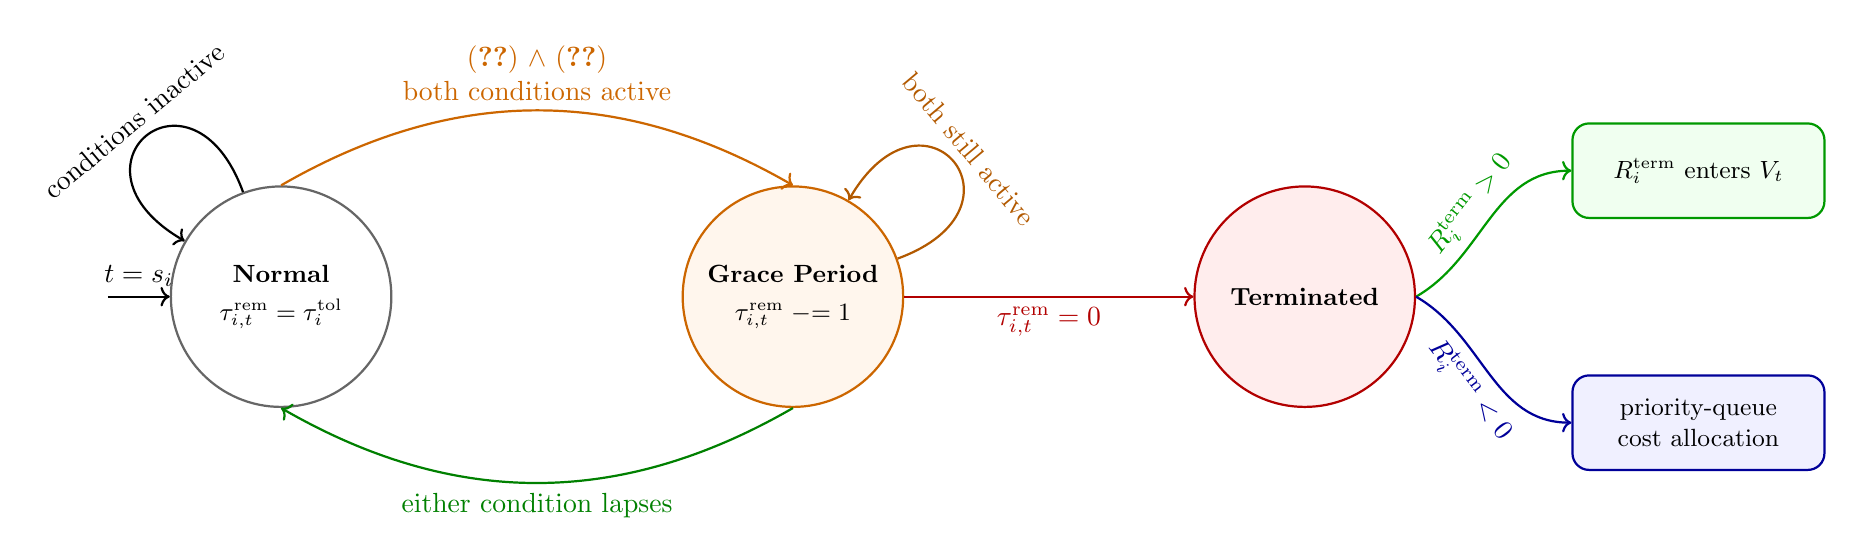
\begin{tikzpicture}[
      every node/.style={font=\small},
      state/.style={circle, draw=black!60, fill=white,
                    minimum size=2.8cm, align=center, thick},
      grace/.style={circle, draw=orange!80!black, fill=orange!7,
                    minimum size=2.8cm, align=center, thick},
      term/.style={circle, draw=red!70!black, fill=red!7,
                    minimum size=2.8cm, align=center, thick},
      posnode/.style={rectangle, rounded corners=6pt, draw=green!60!black,
                  fill=green!6, minimum width=3.2cm, minimum height=1.2cm,
                  align=center, thick},
      negnode/.style={rectangle, rounded corners=6pt, draw=blue!60!black,
                  fill=blue!6, minimum width=3.2cm, minimum height=1.2cm,
                  align=center, thick},
    ]
  
    \node[state] (normal) at (0,0)
      {\textbf{Normal}\\[3pt]
        $\tau_{i,t}^{\mathrm{rem}} = \tau_i^{\mathrm{tol}}$};
  
    \node[grace] (grace) at (6.5,0)
      {\textbf{Grace Period}\\[3pt]
        $\tau_{i,t}^{\mathrm{rem}} \mathrel{-}= 1$};
  
    \node[term] (term) at (13,0)
      {\textbf{Terminated}};
  
    \node[posnode] (posout) at (18,1.6)
      {$R_i^{\mathrm{term}}$ enters $V_t$};
  
    \node[negnode] (negout) at (18,-1.6)
      {priority-queue\\cost allocation};
  
    \draw[->, thick] (-2.2,0) -- (normal.west)
      node[midway, above, font=\normalsize] {$t = s_i$};
  
    \draw[->, thick, orange!80!black]
      (normal.north) to[out=30, in=150]
      node[above, font=\normalsize, align=center]
        {(\ref{eq:term_cond1}) $\wedge$ (\ref{eq:term_cond2})\\both conditions active}
      (grace.north);
  
    \draw[->, thick, green!50!black]
      (grace.south) to[out=210, in=330]
      node[below, font=\normalsize, align=center]
        {either condition lapses}
      (normal.south);
  
    \draw[->, thick, orange!70!black]
      (grace) to[out=20, in=60, looseness=5]
      node[above, font=\normalsize, sloped]
        {both still active}
      (grace);
  
    \draw[->, thick, red!70!black] (grace.east) -- (term.west)
      node[midway, below, font=\normalsize, align=center]
        {$\tau_{i,t}^{\mathrm{rem}} = 0$};
  
    \draw[->, thick, black]
      (normal) to[out=110, in=150, looseness=5]
      node[above, font=\normalsize, sloped] {conditions inactive}
      (normal);
  
    \draw[->, thick, green!60!black]
      (term.east) to[out=30, in=180]
      node[midway, above, font=\normalsize, sloped]
        {$R_i^{\mathrm{term}} > 0$}
      (posout.west);
  
    \draw[->, thick, blue!60!black]
      (term.east) to[out=-30, in=180]
      node[midway, below, font=\normalsize, sloped]
        {$R_i^{\mathrm{term}} < 0$}
      (negout.west);
  
  \end{tikzpicture}%
  }
  \caption{Finite-state representation of the termination mechanic for project $i$.}
  \label{fig:state_machine}
  \end{figure}

Upon termination at $t_i^{\mathrm{term}}$, the net settlement is:
\begin{equation}
  R_i^{\mathrm{term}}
    = P_{i,t_i^{\mathrm{term}}}^{\mathrm{actual}} \cdot CP_i (1-\rho_i)
      - \Bigl(A_i - \sum_{j \in \mathcal{M}_i^{\mathrm{cert}}(t_i^{\mathrm{term}})}
                \delta_i^{\mathrm{rec}} \cdot \phi_{i,j} \cdot CP_i
                \cdot \mathbf{1}\!\left\{\sum_{k \leq j} \phi_{i,k} \geq \psi_i\right\}
        \Bigr).
  \label{eq:term_settlement}
\end{equation}
Negative $R_i^{\mathrm{term}}$ (outstanding advance exceeds earned value)
constitutes a net obligation recovered from portfolio inflows, consistent with
FIDIC termination clauses \citep{FIDIC2017}.

\paragraph{Portfolio cash balance recursion.}
\begin{equation}
  B_{t+1} = B_t
    - \sum_{i \in \mathcal{P}_t^{\mathrm{active}}} x_{i,t}
    + V_t,
  \qquad B_t \geq 0 \quad \forall\,t \in \mathcal{T}.
  \label{eq:balance}
\end{equation}
The constraint $B_t \geq 0$ prohibits borrowing; the portfolio operates under
a fixed capital commitment \cite{kavadias2003resource}. The shared balance $B_t$
is the sole coupling across otherwise independent project dynamics, and its
linear scaling with $n$ characterizes the complexity that motivates the
intractability argument in Level~2.

% - - - - - - - - - - - - - - - - - - - - - - - - - - - - - -
\subsubsection{Shared Objective}
\label{subsubsec:objective}
% - - - - - - - - - - - - - - - - - - - - - - - - - - - - - -

The decision-maker maximizes discounted net cash flow over the horizon:
\begin{equation}
  \max_{\{x_{i,t}\}} \quad
  \mathbb{E}\!\left[
    \sum_{t=1}^{H} \gamma^{t-1}
    \!\left(
      V_t
      - \sum_{i \in \mathcal{P}_t^{\mathrm{active}}} x_{i,t}
      - \sum_{i \in \mathcal{P}_t^{\mathrm{active}}} c_{i,t}^{\mathrm{dev}}
    \right)
  \right],
  \label{eq:objective}
\end{equation}
subject to, for all $i \in \mathcal{P}$, $t \in \mathcal{T}$:
\begin{align}
  x_{i,t} &\geq 0,
  \label{eq:nonnegativity} \\
  \sum_{i \in \mathcal{P}_t^{\mathrm{active}}} x_{i,t} &\leq B_t,
  \label{eq:budget} \\
  x_{i,t} &= 0 \quad \text{if } \mathrm{status}_{i,t} \neq \texttt{active}.
  \label{eq:inactive}
\end{align}
There is no terminal sum. Completion incentives are embedded structurally:
$R_i^{\mathrm{ret}}$ and $R_{i,M_i}^{\mathrm{net}}$ enter $V_t$ at the
certification period; $R_i^{\mathrm{term}}$ (possibly negative) enters at
termination, creating a natural deterrent against allowing project performance
to deteriorate to the termination threshold.
Constraint~\eqref{eq:inactive} enforces that no budget is directed to
completed or terminated projects; the agent is free to allocate any
non-negative amount to active projects subject only to the shared
liquidity constraint~\eqref{eq:budget}.
The expectation $\mathbb{E}[\cdot]$ collapses to a deterministic
evaluation at Level~1 and is retained at Levels~2 and~3.

% ------------------------------------------------------------
\subsection{Level~1: Deterministic Full-Foresight MILP}
\label{subsec:level1}
% ------------------------------------------------------------

Setting $\eta_{i,t} = \bar{\eta}_{i,t}$ (known) renders $S_t$ a deterministic
function of $\mathbf{x}_t$, so $\mathcal{P}_t^{\mathrm{active}}$,
milestone certification times, and termination periods $t_i^{\mathrm{term}}$
are all computable ex ante. Introducing the certification binary
$u_{i,j,t} \in \{0,1\}$ ($=1$ iff milestone $j$ of project $i$ certified by
period $t$) and activity indicator $\mathrm{act}_{i,t} \in \{0,1\}$ (fixed
parameter), the stochastic objective~\eqref{eq:objective} collapses to the MILP:

\begin{subequations}
\label{eq:L1}
\begin{align}
  \max \quad
  & \sum_{t=1}^{H} \gamma^{t-1}\!\left(
      V_t^{\mathrm{det}}
      - \sum_{i \in \mathcal{P}} \mathrm{act}_{i,t}\, x_{i,t}
      - \sum_{i \in \mathcal{P}} \mathrm{act}_{i,t}\, c_{i,t}^{\mathrm{dev}}
    \right)
  \label{eq:L1_obj} \\[4pt]
%
  \text{s.t.} \quad
  B_{t+1} &= B_t
    - \sum_i \mathrm{act}_{i,t}\,x_{i,t} + V_t^{\mathrm{det}},
    \quad B_t \geq 0,
    && \forall\, t
  \label{eq:L1_balance} \\
%
  \sum_i \mathrm{act}_{i,t}\, x_{i,t} &\leq B_t,
    && \forall\, t
  \label{eq:L1_budget} \\
%
  P_{i,t}^{\mathrm{actual}}
    &= P_{i,t-1}^{\mathrm{actual}}
       + \bar{\eta}_{i,t}\,\tfrac{x_{i,t}}{\mathrm{BAC}_i},
    \quad P_{i,t}^{\mathrm{actual}} \leq 1,
    && \forall\, i,t
  \label{eq:L1_progress} \\
%
  P_{i,t}^{\mathrm{actual}}
    &\geq \theta_{i,j}\,u_{i,j,t} - \mathbf{M}(1 - u_{i,j,t}),
    && \forall\, i,j,t
  \label{eq:L1_cert_lb} \\
  P_{i,t}^{\mathrm{actual}}
    &\leq \theta_{i,j} + \mathbf{M}\,u_{i,j,t},
    \quad u_{i,j,t} \geq u_{i,j,t-1},
    \quad u_{i,j+1,t} \leq u_{i,j,t},
    && \forall\, i,j,t
  \label{eq:L1_cert_logic} \\
%
  V_t^{\mathrm{det}}
    &= \sum_{i,j} R_{i,j}^{\mathrm{net}}\,(u_{i,j,t} - u_{i,j,t-1})
       + \sum_i R_i^{\mathrm{ret}}\,(u_{i,M_i,t} - u_{i,M_i,t-1}) \notag \\
    &\quad + \sum_i A_i \cdot \mathbf{1}\{t{=}s_i\}
       + \sum_{i \in \mathcal{P}^{\mathrm{term}}} R_i^{\mathrm{term}}
         \cdot \mathbf{1}\{t{=}t_i^{\mathrm{term}}\},
    && \forall\, t
  \label{eq:L1_cashflow} \\
%
  \delta_{i,t}
    &= P_{i,t}^{\mathrm{actual}} - P_{i,t}^{\mathrm{plan}}
     = d_{i,t}^+ - d_{i,t}^-,
    \quad d_{i,t}^+, d_{i,t}^- \geq 0,
    && \forall\, i,t
  \label{eq:L1_dev_split} \\
  c_{i,t}^{\mathrm{dev}}
    &\geq \lambda_i(d_{i,t}^+ + d_{i,t}^-),
    \quad c_{i,t}^{\mathrm{dev}} \leq \Lambda_i \cdot CP_i,
    \quad c_{i,t}^{\mathrm{dev}} \geq 0,
    && \forall\, i,t
  \label{eq:L1_penalty_lin} \\
%
  x_{i,t}
    &= 0 \quad \text{if } \mathrm{act}_{i,t} = 0,
    && \forall\, i,t
  \label{eq:L1_inactive} \\
%
  x_{i,t} &\geq 0, \quad u_{i,j,t} \in \{0,1\},
    \quad u_{i,j,0} = P_{i,0}^{\mathrm{actual}} = 0.
    &&
  \label{eq:L1_domains}
\end{align}
\end{subequations}

The big-$M$ constant in \eqref{eq:L1_cert_lb}--\eqref{eq:L1_cert_logic}
is $\mathbf{M} = \max_{i,j}\theta_{i,j}$; tighter values may be derived
project-specifically. Constraints~\eqref{eq:L1_cert_lb}--\eqref{eq:L1_cert_logic}
implement the exact if-and-only-if certification logic with monotone, ordered
binary activation. Constraints~\eqref{eq:L1_dev_split}--\eqref{eq:L1_penalty_lin}
linearize the absolute-value and cap in \eqref{eq:penalty}: the maximizing
objective drives $c_{i,t}^{\mathrm{dev}}$ to the tighter of the two bounds,
recovering the exact symmetric penalty. The difference
$(u_{i,j,t} - u_{i,j,t-1})$ in \eqref{eq:L1_cashflow} equals one in the sole
period a milestone is first certified, linearizing the trigger without
additional binaries. Termination timing $t_i^{\mathrm{term}}$ and the
settlement $R_i^{\mathrm{term}}$ (\ref{eq:term_settlement}) are pre-computed
from $\bar{\eta}_{i,t}$ before solving: under deterministic efficiency, the
trajectories of $\mathrm{SPI}_{i,t}$, $\mathrm{CPI}_{i,t}$, and therefore
the counter $\tau_{i,t}^{\mathrm{rem}}$ are fully determined ex ante, so
both termination conditions \eqref{eq:term_cond1}--\eqref{eq:term_cond2}
and the counter dynamics \eqref{eq:counter} are parameter-verifiable at
Level~1. Termination periods and settlements enter the MILP as fixed
parameters rather than optimisation constraints, a simplification that
does not carry over to Levels~2--3 where termination timing is endogenous
to the stochastic trajectory.

\paragraph{Upper bound.}
Let $Z^*_{\mathrm{L1}}$ denote the Level~1 optimum. For any causal policy
$\pi$ feasible under uncertainty, $\sup_\pi \mathbb{E}[Z^\pi] \leq
Z^*_{\mathrm{L1}}$: every feasible causal allocation sequence is also feasible
in the Level~1 program solved on the realized trajectory, so the full-foresight
optimum dominates in expectation. The gap
$Z^*_{\mathrm{L1}} - Z^\pi$ quantifies the cost of uncertainty and anchors the
empirical comparison in Section~\ref{sec:experiments}.

\FloatBarrier

% ============================================================
%  EXPERIMENTS  (uncomment when ready)
% ============================================================

% \section{Experiments}
% \label{sec:experiments}
% \subsection{Overview of the Proposed Solution Framework}
\label{subsec:solution_framework}
% Explain synthetic generator + simulation environment + PPO agent.

\subsection{Literature-Calibrated Synthetic Portfolio Generation}
\label{subsec:synthetic_portfolio_generation}
% Explain how portfolio/project attributes are sampled and calibrated.

\subsection{Environment Initialization}
\label{subsec:environment_initialization}
% Explain reset, initial liquidity, active projects, generated portfolio.

\subsection{MDP Specification}
\label{subsec:mdp_specification}
% Define S, A, P, R, gamma, T.

\subsection{State Representation}
\label{subsec:state_representation}
% Exact state variables and normalization.

\subsection{Action Space and Feasibility Handling}
\label{subsec:action_space}
% Exact allocation action, scaling, clipping, constraints.

\subsection{Transition Dynamics}
\label{subsec:transition_dynamics}
% Progress, SPI/CPI, milestone, cash-flow, liquidity update.

\subsection{Reward Function}
\label{subsec:reward_function}
% Reward components and weights.

\subsection{PPO Training Procedure}
\label{subsec:ppo_training}
% PPO objective, architecture, hyperparameters, training setup.

\subsection{Benchmark Policies and Evaluation Metrics}
\label{subsec:benchmark_evaluation}
% Baselines and metrics.

\subsection{Forward Policy Rollout}
\label{subsec:forward_policy_rollout}
% 12-step simulated trajectory demonstration.


\FloatBarrier

% ============================================================
%  CONCLUSION  (uncomment when ready)
% ============================================================

% \section{Conclusion}
% \label{sec:conclusion}
% \subsection{Summary of Contributions}

This paper establishes the foundational methodology for Reinforcement Learning-based project portfolio budgeting under cashflow uncertainty. Our work addresses a critical gap in operations research: the inability of classical optimization methods to handle sequential decision-making under partial observability in portfolio management.

We make four primary contributions:

\textbf{(1) Literature-Calibrated Synthetic Data Generation:} We developed a comprehensive framework for generating realistic project portfolios with empirically-grounded uncertainty distributions. All parameters are calibrated from published studies (318 megaprojects, multiple empirical analyses), ensuring scientific validity while addressing confidentiality constraints.

\textbf{(2) Rolling Horizon Control Architecture:} We proposed a rolling horizon framework that maintains fixed 12-period episodes while handling variable-duration portfolios through sequential re-planning, preventing state-space explosion and enabling tractable RL training.

\textbf{(3) Formal Problem Formulation:} We provided the first rigorous mathematical formulation of portfolio budgeting as a POMDP with explicit state space, action space, transition dynamics, and reward function, all grounded in empirical project management literature.

\textbf{(4) Complete Modeling Framework:} We documented a modular portfolio modeling system covering composition, cashflows, uncertainty, and revenue plans, with all assumptions explicitly stated and future extensions identified.

\subsection{Implications for Research and Practice}

\textbf{For Operations Research:} This work demonstrates that RL can address problems where classical OR methods fail due to unknown transition probabilities and computational intractability. The rolling horizon architecture provides a template for applying RL to other long-horizon sequential decision problems.

\textbf{For Project Management:} The literature-calibrated synthetic data methodology enables reproducible research in domains with confidentiality constraints. Our framework can be extended to construction, infrastructure, R\&D, and other project-intensive industries.

\textbf{For Machine Learning:} This application showcases RL's potential in operations research domains, complementing recent successes in robotics, game playing, and control. The integration of domain knowledge (S-curves, milestone payments, SPI/CPI dynamics) with data-driven learning exemplifies hybrid AI approaches.

\subsection{Limitations and Scope Boundaries}

We deliberately adopted the \textit{Simplest Model Principle} to establish a foundational framework. Key limitations include:

\begin{itemize}
    \item \textbf{Aggregated cashflow modeling:} No resource-level detail (labor, materials, equipment)
    \item \textbf{Fixed portfolio composition:} 60/40 domestic/international mix assumed optimal
    \item \textbf{Milestone-based payments only:} Alternative structures (time-based, cost-plus) excluded
    \item \textbf{No project interdependencies:} Shared resources and technology spillovers not modeled
    \item \textbf{Synthetic data only:} Real-world validation pending company partnerships
\end{itemize}

Each limitation represents a natural extension for future work, documented with clear research directions.

\subsection{Future Work}

\textbf{Immediate Next Steps (Current Research):}
\begin{enumerate}
    \item \textbf{RL Agent Implementation:} Select and train policy network (PPO, SAC, or Transformer-based)
    \item \textbf{Baseline Comparison:} Implement MIP, stochastic programming, and greedy heuristics
    \item \textbf{Experimental Evaluation:} Conduct comprehensive experiments across scenarios
    \item \textbf{Sensitivity Analysis:} Analyze robustness to parameter variations
\end{enumerate}

\textbf{Medium-Term Extensions (6--12 Months):}
\begin{enumerate}
    \item \textbf{Fine-Tuning Protocol:} Develop methodology for adapting pretrained models to company-specific data
    \item \textbf{Interpretability Analysis:} Apply attention mechanisms or SHAP values to explain allocation decisions
    \item \textbf{Multi-Objective Optimization:} Extend to Pareto-optimal policies balancing NPV, risk, and strategic alignment
    \item \textbf{Real-World Validation:} Partner with EPC contractors for pilot deployment
\end{enumerate}

\textbf{Long-Term Research Directions (1--3 Years):}
\begin{enumerate}
    \item \textbf{Resource-Level Modeling:} Disaggregate cashflows into labor, materials, equipment with detailed scheduling
    \item \textbf{Dynamic Portfolio Selection:} Integrate project selection with execution optimization
    \item \textbf{Multi-Agent RL:} Model interactions between contractor, client, and subcontractors
    \item \textbf{Transfer Learning:} Investigate cross-domain transfer (oil \& gas $\to$ construction $\to$ infrastructure)
    \item \textbf{Hierarchical RL:} Develop two-level policies (strategic portfolio allocation + tactical project control)
\end{enumerate}

\subsection{Broader Impact}

This research has potential impact beyond project portfolio management:

\textbf{Methodological Contributions:}
\begin{itemize}
    \item Template for applying RL to OR problems with unknown transition dynamics
    \item Framework for literature-calibrated synthetic data generation
    \item Rolling horizon architecture for long-horizon sequential decision problems
\end{itemize}

\textbf{Practical Applications:}
\begin{itemize}
    \item Real-time decision support for portfolio managers
    \item Scenario analysis for strategic planning
    \item Risk assessment through Monte Carlo simulation
    \item Training tool for project management education
\end{itemize}

\textbf{Open Science:}
\begin{itemize}
    \item Complete codebase and datasets released as open source
    \item Reproducible research enabling community validation and extension
    \item Benchmark problem for RL algorithm development
\end{itemize}

\subsection{Concluding Remarks}

Project portfolio budgeting under uncertainty represents a critical challenge for capital-intensive industries. Traditional optimization methods fail due to computational intractability and unknown state transition probabilities. This paper establishes the foundational methodology for addressing this challenge through Reinforcement Learning with rolling horizon control.

By developing a literature-calibrated synthetic data generation framework, we overcome the confidentiality barrier that has prevented progress in this domain. Our formal problem formulation and complete modeling framework provide a rigorous foundation for future research.

The path forward is clear: implement and evaluate RL agents, compare against classical baselines, and develop fine-tuning protocols for company-specific deployment. We invite the research community to build upon this foundation, extending the methodology to related domains and advancing the state of the art in RL-based operations research.

The complete modeling framework, instance generator, and documentation will be released as open-source software upon publication, enabling reproducible research and practical deployment in this emerging field.


\FloatBarrier

% ============================================================
%  ACKNOWLEDGMENTS  (uncomment when ready)
% ============================================================

% \section*{Acknowledgments}
% This research was supported by [Funding Agency].

\FloatBarrier

% ============================================================
%  BIBLIOGRAPHY
% ============================================================

\bibliographystyle{apalike}
\bibliography{references}

\FloatBarrier

% ============================================================
%  APPENDIX A — PRISMA 2020 Flow Diagram
% ============================================================

\newpage
\appendix
\section{Appendix A : PRISMA 2020 Flow Diagram}
\label{app:prisma}
% ================================================================
%  APPENDIX A
% ================================================================
% \vspace{0.5cm}
 
\begin{figure}[htbp]
\centering
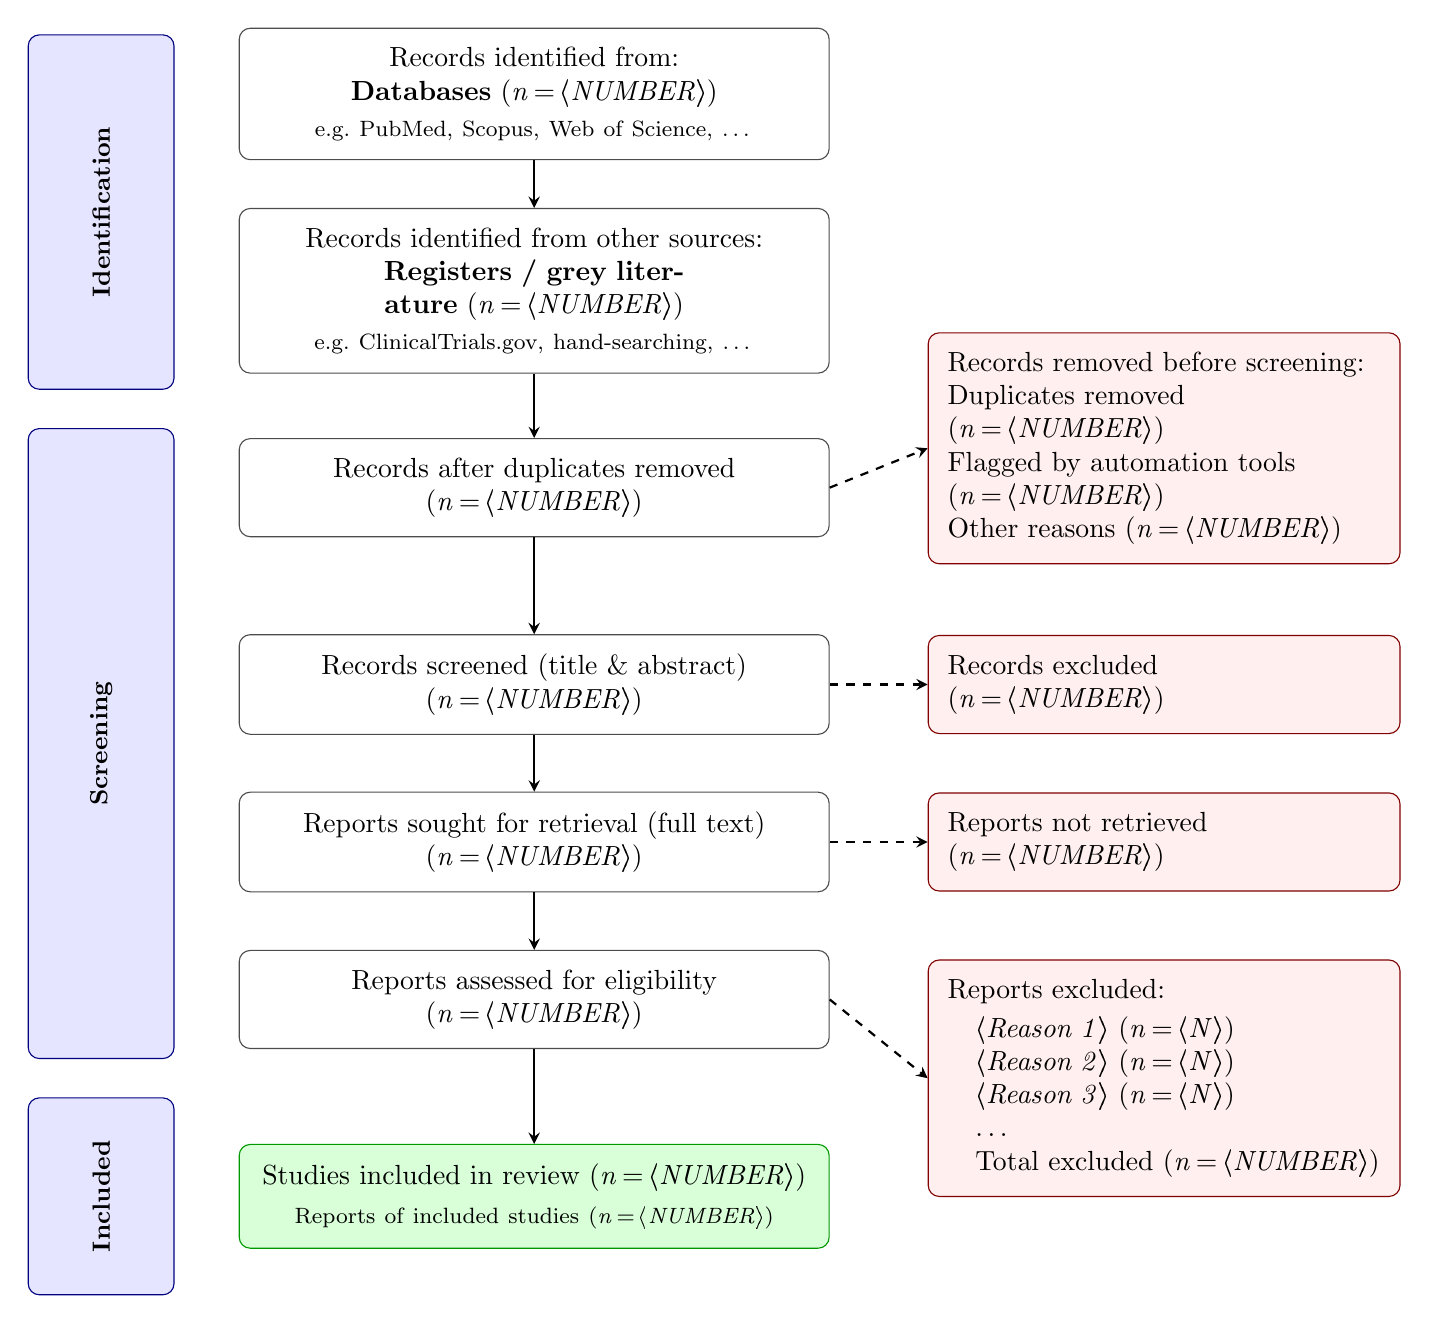
\begin{tikzpicture}
 
% ────────────────────────────────────────────────────────────
%  Row y-positions (generous spacing prevents excl-box overlap)
%
%   id1  :  y =   0
%   id2  :  y =  -3.0
%   sc1  :  y =  -6.5
%   sc2  :  y =  -9.5
%   sc3  :  y = -12.5
%   sc4  :  y = -15.5
%   inc1 :  y = -20.0   (extra gap; exc4 has 6 lines ~4 cm tall)
%
%  Columns
%   phase labels : x = -4.5
%   main flow    : x =  0
%   excl boxes   : x =  9.0
% ────────────────────────────────────────────────────────────
 
% ═══════════════════════════════════════════════════════════
%  IDENTIFICATION  –  phase label spans y=0 to y=-3.0, mid=-1.5
% ═══════════════════════════════════════════════════════════
\node[phase, minimum height=4.5cm] (ph-id) at (-4.5, -1.5)
  {\rotatebox{90}{Identification}};
 
\node[box] (id1) at (1, 0)
  {Records identified from:\\
   \textbf{Databases} (\textit{n}\,=\,\textlangle\textit{NUMBER}\textrangle)\\[1pt]
   \footnotesize e.g.\ PubMed, Scopus, Web of Science, \ldots};
 
\node[box] (id2) at (1, -2.5)
  {Records identified from other sources:\\
   \textbf{Registers / grey literature} (\textit{n}\,=\,\textlangle\textit{NUMBER}\textrangle)\\[1pt]
   \footnotesize e.g.\ ClinicalTrials.gov, hand-searching, \ldots};
 
\draw[arr] (id1.south) -- (id2.north);
 
% ═══════════════════════════════════════════════════════════
%  SCREENING  –  phase label spans y=-6.5 to y=-15.5, mid=-11.0
%                height = 15.5 - 6.5 + 2.0 (padding) = 11.0 cm
% ═══════════════════════════════════════════════════════════
\node[phase, minimum height=8.0cm] (ph-sc) at (-4.5, -8.25)
  {\rotatebox{90}{Screening}};
 
\node[box] (sc1) at (1, -5.0)
  {Records after duplicates removed\\
   (\textit{n}\,=\,\textlangle\textit{NUMBER}\textrangle)};
 
\node[excl] (exc1) at (9.0, -4.5)
  {Records removed before screening:\\
   Duplicates removed (\textit{n}\,=\,\textlangle\textit{NUMBER}\textrangle)\\
   Flagged by automation tools (\textit{n}\,=\,\textlangle\textit{NUMBER}\textrangle)\\
   Other reasons (\textit{n}\,=\,\textlangle\textit{NUMBER}\textrangle)};
 
\draw[arr]  (id2.south) -- (sc1.north);
\draw[arr2] (sc1.east)  -- (exc1.west);
 
\node[box] (sc2) at (1, -7.5)
  {Records screened (title \& abstract)\\
   (\textit{n}\,=\,\textlangle\textit{NUMBER}\textrangle)};
 
\node[excl] (exc2) at (9.0, -7.5)
  {Records excluded\\
   (\textit{n}\,=\,\textlangle\textit{NUMBER}\textrangle)};
 
\draw[arr]  (sc1.south) -- (sc2.north);
\draw[arr2] (sc2.east)  -- (exc2.west);
 
\node[box] (sc3) at (1, -9.5)
  {Reports sought for retrieval (full text)\\
   (\textit{n}\,=\,\textlangle\textit{NUMBER}\textrangle)};
 
\node[excl] (exc3) at (9.0, -9.5)
  {Reports not retrieved\\
   (\textit{n}\,=\,\textlangle\textit{NUMBER}\textrangle)};
 
\draw[arr]  (sc2.south) -- (sc3.north);
\draw[arr2] (sc3.east)  -- (exc3.west);
 
\node[box] (sc4) at (1, -11.5)
  {Reports assessed for eligibility\\
   (\textit{n}\,=\,\textlangle\textit{NUMBER}\textrangle)};
 
\node[excl] (exc4) at (9.0, -12.5)
  {Reports excluded:\\[2pt]
   \quad \textlangle\textit{Reason 1}\textrangle\ (\textit{n}\,=\,\textlangle\textit{N}\textrangle)\\
   \quad \textlangle\textit{Reason 2}\textrangle\ (\textit{n}\,=\,\textlangle\textit{N}\textrangle)\\
   \quad \textlangle\textit{Reason 3}\textrangle\ (\textit{n}\,=\,\textlangle\textit{N}\textrangle)\\
   \quad \ldots\\
   \quad Total excluded (\textit{n}\,=\,\textlangle\textit{NUMBER}\textrangle)};
 
\draw[arr]  (sc3.south) -- (sc4.north);
\draw[arr2] (sc4.east)  -- (exc4.west);
 
% ═══════════════════════════════════════════════════════════
%  INCLUDED  –  phase label centred on y=-20.0
% ═══════════════════════════════════════════════════════════
\node[phase, minimum height=2.5cm] (ph-inc) at (-4.5, -14.0)
  {\rotatebox{90}{Included}};
 
\node[incl] (inc1) at (1, -14.0)
  {Studies included in review
   (\textit{n}\,=\,\textlangle\textit{NUMBER}\textrangle)\\[2pt]
   \footnotesize Reports of included studies
   (\textit{n}\,=\,\textlangle\textit{NUMBER}\textrangle)};
 
\draw[arr] (sc4.south) -- (inc1.north);
 
% ── Optional meta-analysis box – uncomment if needed ────────
%\node[phase, minimum height=2.5cm] at (-4.5, -23.0) {\rotatebox{90}{Included}};
%\node[incl] (inc2) at (0, -23.0)
%  {Studies included in meta-analysis\\
%   (\textit{n}\,=\,\textlangle\textit{NUMBER}\textrangle)};
%\draw[arr] (inc1.south) -- (inc2.north);
 
\end{tikzpicture}
 
\caption{PRISMA 2020 flow diagram of the literature search and
         selection process.}
\label{fig:prisma}
\end{figure}


\FloatBarrier

% ============================================================
%  APPENDIX B — Environment Verification Suite
% ============================================================

\newpage
\appendix
\section{Appendix B : Environment verification suite}
\label{app:env_veri_suit}
The following flow diagram illustrates the systematic literature
search and screening process following the PRISMA 2020 guidelines
\cite{Page2021}.  % replace or remove if not using BibTeX
 
\vspace{0.5cm}
 
\begin{figure}[h!]
\centering
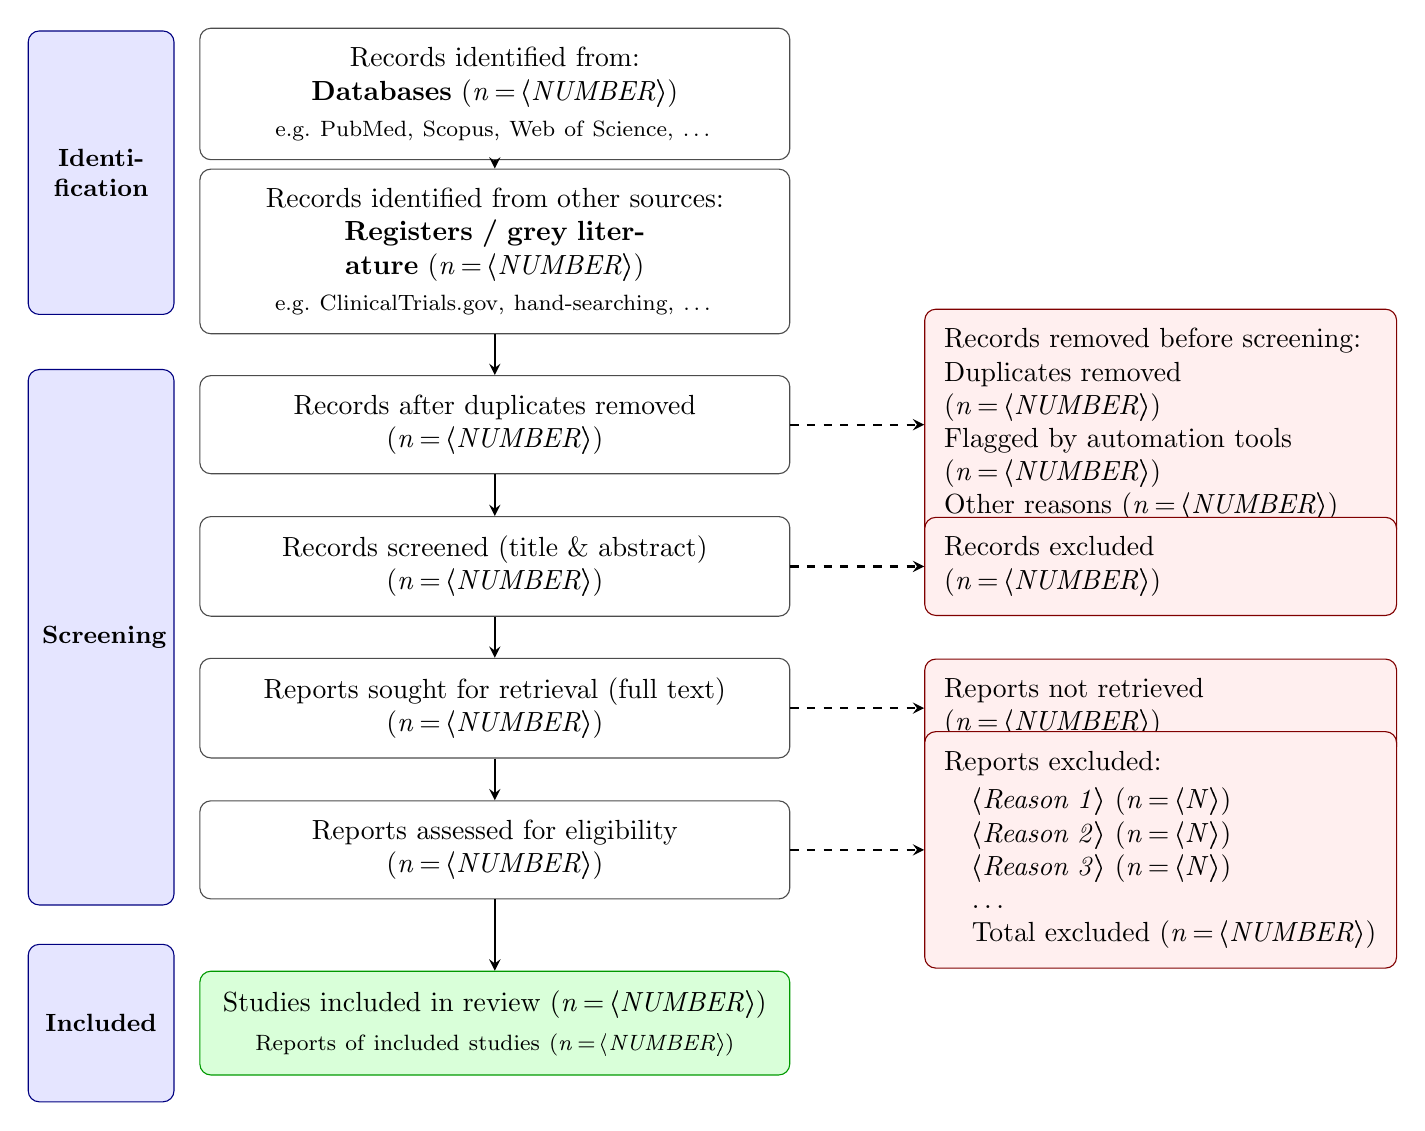
\begin{tikzpicture}
 
% ────────────────────────────────────────────────────────────
%  All nodes use absolute coordinates so phase labels and
%  their content boxes are always vertically centred together.
%
%  Main-flow boxes (col x=0):  id1, id2, sc1–sc4, inc1
%  Phase labels   (col x=-5):  ph-id, ph-sc, ph-inc
%  Exclusion boxes(col x=8.2): exc1–exc4
% ────────────────────────────────────────────────────────────
 
% ── Row y-positions ─────────────────────────────────────────
%   id1  : y =  0
%   id2  : y = -2.0
%   sc1  : y = -4.2
%   sc2  : y = -6.0
%   sc3  : y = -7.8
%   sc4  : y = -9.6
%   inc1 : y = -11.8
 
% ═══════════════════════════════════════════════════════════
%  IDENTIFICATION
% ═══════════════════════════════════════════════════════════
 
% Phase label – vertically centred over id1 and id2
% Centre of id1=0, centre of id2=-2.0  →  mid = -1.0
\node[phase, minimum height=3.6cm] (ph-id) at (-5, -1.0)
  {Identi-\\fication};
 
\node[box] (id1) at (0, 0)
  {Records identified from:\\
   \textbf{Databases} (\textit{n}\,=\,\textlangle\textit{NUMBER}\textrangle)\\[1pt]
   \footnotesize e.g.\ PubMed, Scopus, Web of Science, \ldots};
 
\node[box] (id2) at (0, -2.0)
  {Records identified from other sources:\\
   \textbf{Registers / grey literature} (\textit{n}\,=\,\textlangle\textit{NUMBER}\textrangle)\\[1pt]
   \footnotesize e.g.\ ClinicalTrials.gov, hand-searching, \ldots};
 
\draw[arr] (id1.south) -- (id2.north);
 
% ═══════════════════════════════════════════════════════════
%  SCREENING
% ═══════════════════════════════════════════════════════════
 
% Phase label – centred over sc1(−4.2) through sc4(−9.6)  →  mid = −6.9
\node[phase, minimum height=6.8cm] (ph-sc) at (-5, -6.9)
  {Screening};
 
\node[box] (sc1) at (0, -4.2)
  {Records after duplicates removed\\
   (\textit{n}\,=\,\textlangle\textit{NUMBER}\textrangle)};
 
\node[excl, right=1.7cm of sc1] (exc1)
  {Records removed before screening:\\
   Duplicates removed (\textit{n}\,=\,\textlangle\textit{NUMBER}\textrangle)\\
   Flagged by automation tools (\textit{n}\,=\,\textlangle\textit{NUMBER}\textrangle)\\
   Other reasons (\textit{n}\,=\,\textlangle\textit{NUMBER}\textrangle)};
 
\draw[arr]  (id2.south) -- (sc1.north);
\draw[arr2] (sc1.east)  -- (exc1.west);
 
\node[box] (sc2) at (0, -6.0)
  {Records screened (title \& abstract)\\
   (\textit{n}\,=\,\textlangle\textit{NUMBER}\textrangle)};
 
\node[excl, right=1.7cm of sc2] (exc2)
  {Records excluded\\
   (\textit{n}\,=\,\textlangle\textit{NUMBER}\textrangle)};
 
\draw[arr]  (sc1.south) -- (sc2.north);
\draw[arr2] (sc2.east)  -- (exc2.west);
 
\node[box] (sc3) at (0, -7.8)
  {Reports sought for retrieval (full text)\\
   (\textit{n}\,=\,\textlangle\textit{NUMBER}\textrangle)};
 
\node[excl, right=1.7cm of sc3] (exc3)
  {Reports not retrieved\\
   (\textit{n}\,=\,\textlangle\textit{NUMBER}\textrangle)};
 
\draw[arr]  (sc2.south) -- (sc3.north);
\draw[arr2] (sc3.east)  -- (exc3.west);
 
\node[box] (sc4) at (0, -9.6)
  {Reports assessed for eligibility\\
   (\textit{n}\,=\,\textlangle\textit{NUMBER}\textrangle)};
 
\node[excl, right=1.7cm of sc4] (exc4)
  {Reports excluded:\\[2pt]
   \quad \textlangle\textit{Reason 1}\textrangle\ (\textit{n}\,=\,\textlangle\textit{N}\textrangle)\\
   \quad \textlangle\textit{Reason 2}\textrangle\ (\textit{n}\,=\,\textlangle\textit{N}\textrangle)\\
   \quad \textlangle\textit{Reason 3}\textrangle\ (\textit{n}\,=\,\textlangle\textit{N}\textrangle)\\
   \quad \ldots\\
   \quad Total excluded (\textit{n}\,=\,\textlangle\textit{NUMBER}\textrangle)};
 
\draw[arr]  (sc3.south) -- (sc4.north);
\draw[arr2] (sc4.east)  -- (exc4.west);
 
% ═══════════════════════════════════════════════════════════
%  INCLUDED
% ═══════════════════════════════════════════════════════════
 
% Phase label – centred on inc1 at y=−11.8
\node[phase, minimum height=2.0cm] (ph-inc) at (-5, -11.8)
  {Included};
 
\node[incl] (inc1) at (0, -11.8)
  {Studies included in review
   (\textit{n}\,=\,\textlangle\textit{NUMBER}\textrangle)\\[2pt]
   \footnotesize Reports of included studies
   (\textit{n}\,=\,\textlangle\textit{NUMBER}\textrangle)};
 
\draw[arr] (sc4.south) -- (inc1.north);
 
% ── Optional meta-analysis box – uncomment if needed ────────
%\node[incl] (inc2) at (0, -13.6)
%  {Studies included in meta-analysis\\
%   (\textit{n}\,=\,\textlangle\textit{NUMBER}\textrangle)};
%\draw[arr] (inc1.south) -- (inc2.north);
%\node[phase, minimum height=2.0cm] at (-5,-13.6) {Included};
 
\end{tikzpicture}
 
\caption{PRISMA 2020 flow diagram of the literature search and
         selection process.}
\label{fig:prisma}
\end{figure}
 
{\footnotesize
\textbf{Note.} Adapted from Page et al.\ (2021). \textit{The PRISMA
2020 statement: an updated guideline for reporting systematic
reviews.} \textit{BMJ}, 372, n71.
}

\FloatBarrier

% ============================================================
%  APPENDIX C — Instance Generator Algorithm  (uncomment when ready)
% ============================================================

% \section{Instance Generator Algorithm}
% \label{app:algorithm}
% \subsection{Instance Generator Algorithm}

This appendix provides the complete pseudocode for the portfolio instance generator.

\begin{algorithm}[H]
\caption{Portfolio Instance Generator}
\label{alg:instance_generator}
\begin{algorithmic}[1]
\Require Portfolio size range $[N_{\min}, N_{\max}]$, parameter tables
\Ensure Portfolio instance $\mathcal{P}$ with all attributes
\State
\State \textbf{Stage 1: Portfolio Composition}
\State $N \gets \text{UniformInt}(N_{\min}, N_{\max})$
\State $N_{\text{domestic}} \gets \lfloor 0.6 \times N \rfloor$
\State $N_{\text{international}} \gets N - N_{\text{domestic}}$
\State
\State \textbf{Stage 2: Project Characteristics}
\For{$i = 1$ to $N$}
    \State Assign category: domestic or international
    \State Sample $\log(\text{BAC}_i) \sim \mathcal{N}(\mu_{\log}, \sigma_{\log})$
    \State Clip $\text{BAC}_i$ to $[\$50M, \$5B]$
    \State Sample $\pi_i \sim \text{TruncatedNormal}(\mu_\pi, \sigma_\pi, a_\pi, b_\pi)$
    \State Compute $R_i \gets \text{BAC}_i \times (1 + \pi_i)$
    \State Sample $D_i \gets D_{\text{base}} \times (\text{BAC}_i / \text{BAC}_{\text{ref}})^{0.35} \times \epsilon_D$
    \State Clip $D_i$ to $[12, 60]$ months
\EndFor
\State
\State \textbf{Stage 3: S-Curve Parameters}
\For{$i = 1$ to $N$}
    \State Compute size multiplier: $m_{\text{size}} \gets (\text{BAC}_i / \text{BAC}_{\text{median}})^{0.15}$
    \State Compute duration multiplier: $m_{\text{dur}} \gets (D_i / D_{\text{median}})^{0.12}$
    \State Get category multiplier $m_{\text{cat}}$ (0.9 for domestic, 1.1 for international)
    \State Sample risk level: low or high
    \State Get risk multipliers $m_{\text{risk}}^\alpha$, $m_{\text{risk}}^\beta$
    \State Sample $\epsilon_\alpha, \epsilon_\beta \sim \text{LogNormal}(0, 0.10)$
    \State $\alpha_i \gets \alpha_{\text{base}} \times m_{\text{size}} \times m_{\text{cat}} \times m_{\text{risk}}^\alpha \times \epsilon_\alpha$
    \State $\beta_i \gets \beta_{\text{base}} \times m_{\text{dur}} \times m_{\text{cat}} \times m_{\text{risk}}^\beta \times \epsilon_\beta$
    \State Clip $\alpha_i$ to $[1.2, 5.0]$, $\beta_i$ to $[1.2, 5.5]$
\EndFor
\State
\State \textbf{Stage 4: Cashflow Profiles}
\For{$i = 1$ to $N$}
    \For{$t = 0$ to $D_i$}
        \State $\tau \gets t / D_i$
        \State $S_i(t) \gets \text{BAC}_i \times I_\tau(\alpha_i, \beta_i)$ \Comment{Cumulative spending}
        \State $c_i(t) \gets S_i(t) - S_i(t-1)$ \Comment{Incremental cashflow}
    \EndFor
\EndFor
\State
\State \textbf{Stage 5: Performance Uncertainty}
\State Sample $(u_{\text{SPI}}, u_{\text{CPI}}) \sim \text{BivariateNormal}(\rho = 0.68)$
\For{$i = 1$ to $N$}
    \State $v_{\text{SPI}} \gets \Phi(u_{\text{SPI}}^i)$, $v_{\text{CPI}} \gets \Phi(u_{\text{CPI}}^i)$
    \State $\text{SPI}_i \gets 0.3 + 1.0 \times \text{Beta}^{-1}(v_{\text{SPI}}; 2.8, 2.2)$
    \State $\text{CPI}_i \gets 0.5 + 0.7 \times \text{Beta}^{-1}(v_{\text{CPI}}; 3.2, 1.8)$
\EndFor
\State
\State \textbf{Stage 6: Revenue Plans}
\For{$i = 1$ to $N$}
    \State Define milestones: $\{(p_m, w_m)\}$ for $m = 0, 1, \ldots, M$
    \State Compute milestone payments: $R_i^m \gets R_i \times w_m$
    \State Compute planned milestone times: $t_m^{\text{plan}} \gets D_i \times p_m$
    \State Store milestone structure for project $i$
\EndFor
\State
\State \Return Portfolio instance $\mathcal{P} = \{(\text{BAC}_i, D_i, \pi_i, R_i, \alpha_i, \beta_i, \text{SPI}_i, \text{CPI}_i, \text{milestones}_i)\}_{i=1}^N$
\end{algorithmic}
\end{algorithm}

\subsection{Validation Algorithm}

\begin{algorithm}[H]
\caption{Instance Validation}
\label{alg:validation}
\begin{algorithmic}[1]
\Require Generated portfolio instance $\mathcal{P}$, target statistics
\Ensure Validation report (pass/fail for each check)
\State
\State \textbf{Level 1: Distributional Validation}
\For{each variable $X$ in $\{\text{BAC}, \pi, D, \alpha, \beta, \text{SPI}, \text{CPI}\}$}
    \State Compute sample mean $\bar{X}$, std dev $s_X$
    \State Check: $|\bar{X} - \mu_{\text{target}}| / \mu_{\text{target}} < 0.05$ \Comment{5\% tolerance}
    \State Check: $|s_X - \sigma_{\text{target}}| / \sigma_{\text{target}} < 0.10$ \Comment{10\% tolerance}
\EndFor
\State
\State \textbf{Level 2: Correlation Validation}
\State Compute $\rho(\text{SPI}, \text{CPI})$
\State Check: $|\rho - 0.68| < 0.05$
\State
\State \textbf{Level 3: Portfolio-Level Validation}
\State Compute total portfolio BAC: $\sum_{i=1}^N \text{BAC}_i$
\State Compute domestic fraction: $\sum_{i \in \text{domestic}} \text{BAC}_i / \sum_{i=1}^N \text{BAC}_i$
\State Check: domestic fraction $\in [0.55, 0.65]$ \Comment{60\% $\pm$ 5\%}
\State
\State \textbf{Level 4: Sanity Checks}
\For{$i = 1$ to $N$}
    \State Check: $\text{BAC}_i > 0$, $D_i > 0$, $\pi_i > 0$
    \State Check: $\alpha_i \in [1.2, 5.0]$, $\beta_i \in [1.2, 5.5]$
    \State Check: $\text{SPI}_i \in [0.3, 1.3]$, $\text{CPI}_i \in [0.5, 1.2]$
    \State Check: $\sum_m w_m = 1.0$ \Comment{Milestone weights sum to 100\%}
\EndFor
\State
\State \Return Validation report
\end{algorithmic}
\end{algorithm}

\subsection{Implementation Notes}

\textbf{Computational Complexity:} The instance generator has time complexity $O(N \times D_{\max})$ where $N$ is portfolio size and $D_{\max}$ is maximum project duration. For typical values ($N=15$, $D_{\max}=60$), generation takes $<$1 second per instance.

\textbf{Reproducibility:} All random number generation uses seeded PRNGs (NumPy default\_rng with explicit seeds). Seeds are logged for each generated instance.

\textbf{Parallelization:} Instance generation is embarrassingly parallel. For large datasets (10,000+ instances), use multiprocessing with one worker per CPU core.

\textbf{Output Format:} Instances are serialized as JSON or HDF5 files with standardized schema for interoperability.


\end{document}